
%--------------------
 
\chapter{Modelos empíricos y jerárquicos}

En las últimas décadas la formulación de modelos estadísticos ha evolucionado mucho En un principio, los modelos establecidos obedecían a reglas estándares que se suponían ciertas para toda la población. Sin embargo, el estado de la naturaleza de la mayoría de los problemas práctico no sigue una regla común para todos y cada uno de los elementos de una población aleatoria. De hecho el sentido común establece que para una misma población, pueden existir tendencias comunes entre diferentes miembros de la misma y la estructura de dispersión de los elementos puede obedecer comportamientos disímiles a través de éstos.

Lo anterior ha permitido que el investigador pueda proponer modelos que siguen comportamientos estructurales distintos y en algunos casos que se encuentran anidados en modelos más complejos. En el caso bayesiano, es claro que el momento de coyuntura en el cual el investigador no contempla un punto de retorno está dado en la formulación de la distribución previa para el vector de parámetros de interés $\btheta$. Más aún, la influencia de la distribución previa en la resultante distribución posterior está dada por la asignación del vector de hiperparámetros $\bEta$ que parametriza la distribución previa. Cuando los valores exactos de los hiperparámetros se desconocen o cuando no se tiene plena certeza del comportamiento estructural de la distribución previa, entonces es necesario estimarlos pues de estos dependen los resultados en cualquier investigación de tipo causal. En otras palabras, una mala asignación de los valores de los hiperparámetros conduce a una distribución previa que no es acorde con la realidad y esto puede conllevar a su vez a que la distribución posterior no concuerde con la realidad, produciendo así resultados engañosos.

Siguiendo los fundamentos filosóficos de la estadística bayesiana, tener que estimar el vector de hiperparámetros envuelve al investigador en una paradoja cuya solución no siempre está dada por métodos bayesianos. En primer lugar, nótese la forma de la distribución previa del vector de parámetros de interés: $p(\btheta \mid \bEta)$. A simple vista se puede concluir que $\bEta$ hace parte de la distribución previa la cual, según la lógica de la filosofía bayesiana, involucra el conocimiento del investigador antes de la recolección de los datos. Por tanto la pregunta directa que surge es ¿Por qué estimar algo que se debería suponer conocido?. En segundo lugar y si se concibe tal estimación, la otra pregunta natural es ¿Se deben utilizar los datos para estimar tales hiperparámetros?. Las posibles respuestas a las anteriores preguntas han creado toda una nueva corriente alterna a la bayesiana pura llamada <<corriente bayesiana empírica>>\footnote{\citeasnoun{Carlin96} menciona que el análisis empírico toma este nombre por dos razones: En primer lugar porque estima el vector de hiper-parámetros $\bEta$ con los datos observados, contradiciendo de alguna manera el espíritu y la filosofía de la corriente bayesiana radical. En segundo lugar, porque esta estimación se realiza con métodos frecuentistas ya sean paramétricos o no-paramétricos} la cual utiliza los métodos de estimación puntual frecuentista para estimar estos hiperparámetros y por consiguiente definir la distribución previa del vector de parámetros de interés.

LADY TASTING TEA SOBRE EMPIRICAL Y BAYES

Por supuesto, existe la contraparte teórica a la corriente empírica y es la llamada <<corriente bayesiana jerárquica>> la cual asume una posición totalmente bayesiana desde su concepción y establece un modelo posterior para los hiperparámetros.

Suponga entonces que la variable de interés sigue un modelo común a toda la población aunque parametrizado por parámetros que toman distintos valores para cada individuo y que está regido por la siguiente expresión
\begin{equation*}
Y_i\sim p(Y_i \mid \theta_i)
\end{equation*}

\section{Análisis empírico}

COLOCAR LOS TIPOS DE ANÁLISIS: PARAMÉTRICO Y NO PARAMÉTRICO Y LOS PRINCIPALES RESULTADOS

Este enfoque, criticado por muchos bayesianos radicales, se centra en la escogencia de una estimación $\hat{\bEta}$ de $\bEta$ obtenida como el valor que hace maxima la verosimilitud marginal previa dada por
\begin{align}\label{ecua1}
p(\mathbf{Y} \mid \bEta)=\int p(\mathbf{Y} \mid \btheta)p(\btheta \mid \bEta) \ d\btheta
\end{align}

Por lo tanto todo el andamiaje inferencial está supeditado a la distribución posterior estimada, $p(\btheta \mid Y,\hat{\bEta})$. Una vez que ésta esté bien definida, el proceso de estimación puntual, estimación por intervalo y pruebas de hipótesis sigue su curso bayesiano idénticamente como en los capítulos anteriores.

En términos prácticos suponga que se tiene un modelo en dos etapas para cada una de las observaciones. Se asume que existen $n$ observaciones que, si bien no conforman una muestra aleatoria, conservan la característica de intercambiebilidad y están definidas en los siguientes términos
\begin{equation*}
Y_i \sim p(Y_i \mid \theta_i) \ \ \ \ \ \ \ i=1,\ldots,n
\end{equation*}

La segunda etapa comienza con la asignación de una distribución\footnote{En esta etapa la distribución previa no está completamente especificada puesto que se desconocen los hiperparámetros que la indexan.} previa para los parámetros de interés $\theta_i$.
\begin{equation*}
\theta_i \sim p(\theta_i \mid \bEta) \ \ \ \ \ \ \ i=1,\ldots,n
\end{equation*}

Nótese que detrás de la asignación de la estructura probabilística para cada uno de los $\theta_i$, se supone que éstos últimos determinan una muestra aleatoria de la distribución $p(\btheta \mid \bEta)$.
El objetivo de este enfoque es encontrar estimadores que maximicen la verosimilitud marginal previa la cual, para este caso particular y considerando independencia marginal entre las observaciones y el vector de hiperparámetros, es
\begin{align}
p(Y_i \mid \bEta)&=\int p(Y_i,\theta_i \mid \bEta) \ d\theta_i \notag \\
&=\int p(Y_i \mid \theta_i,\bEta)p(\theta_i \mid \bEta) \ d\theta_i \notag \\
&=\int p(Y_i \mid \theta_i)p(\theta_i \mid \bEta) \ d\theta_i
\end{align}

De lo anterior, la verosimilitud marginal previa del vector de observaciones dada por la expresión (\ref{ecua1}) queda convertida en
\begin{align}
p(Y \mid \bEta)&=\prod_{i=1}^np(Y_i \mid \bEta) \notag \\
&=\prod_{i=1}^n\int p(Y_i \mid \theta_i)p(\theta_i \mid \bEta) \ d\theta_i
\end{align}

A continuación, examninamos algunas distribuciones 

\subsection{Modelo Binomial-Beta}\label{Binomial-Beta}
Suponga el siguiente modelo binomial (intercambiable) en una primera etapa
\begin{equation*}
Y_i \mid \theta_i \sim Binomial(n_i,\theta_i)  \ \ \ \ \ \ \ i=1,\ldots,p
\end{equation*}

Para la segunda etapa, se supone una muestra aleatoria (independientes e idénticamente distribuidos) proveniente de una misma distribución tal que
\begin{equation*}
\theta_i \sim Beta(\alpha, \beta)  \ \ \ \ \ \ \ i=1,\ldots,p
\end{equation*}

puesto que cada $\theta_i$ se encuentra en el intervalo $(0,1)$ y es apropiado asignarle una distribución Beta.
\subsubsection{Análisis preliminar}

Es bien sabido que la distribución posterior para cada uno de los parámetros de interés involucrados en el anterior contexto está dada por
\begin{equation*}
\theta_i \mid Y_i \sim Beta(\alpha+Y_i, \beta+n_i-y_i)
\end{equation*}

para todo $i=1,\cdots,p$. Sin embargo, como se desconoce totalmente el valor de los hiperparámetros $\alpha$ y $\beta$, entonces se debe encontrar una estimación de estos, $\hat{\alpha}$ y $\hat{\beta}$, respectivamente, para proseguir normalmente con la inferencia bayesiana, pero esta vez enfocados en la estimación de la distribución posterior dada por
\begin{equation*}
\theta_i \mid Y_i \sim Beta(\hat{\alpha}+Y_i, \hat{\beta}+n_i-y_i)
\end{equation*}

Para tal fin, nótese que la esperanza y la varianza previa de $\theta_i$ están dadas por las siguientes expresiones
\begin{align}
E(\theta_i)&=\frac{\alpha}{\alpha+\beta}\label{ecua2}\\
Var(\theta_i)&=\frac{\alpha\beta}{(\alpha+\beta)^2(\alpha+\beta+1)}\label{ecua3}
\end{align}

De donde se tiene que
\begin{align}\label{ecua5}
\alpha=E(\theta_i)(\alpha+\beta)
\end{align}

y también que
\begin{align}\label{ecua4}
1-E(\theta_i)=\frac{\beta}{\alpha+\beta}
\end{align}

por lo tanto
\begin{align}\label{ecua6}
\beta=(1-E(\theta_i))(\alpha+\beta)
\end{align}

y reemplazando (\ref{ecua2}) y (\ref{ecua4}) en (\ref{ecua3}) se concluye que
\begin{align*}
Var(\theta_i)&=\frac{E(\theta_i)(1-E(\theta_i))}{(\alpha+\beta+1)}
\end{align*}

por tanto
\begin{align}
\alpha+\beta=\frac{E(\theta_i)(1-E(\theta_i))}{Var(\theta_i)}-1
\end{align}

Con el anterior razonamiento, es posible encontrar los estimadores basados en el método frecuentista de los momentos los cuales corresponden a
\begin{align}
\widehat{\alpha+\beta}&=\frac{\bar{Y}(1-\bar{Y})}{S^2}-1
\end{align}

Donde $\bar{Y}$ y $S^2$ es el promedio y la varianza de las cantidades $Y_1/n_1, Y_2/n_2,\ldots, Y_p/n_p$, respectivamente. Ahora, teniendo en cuenta que (\ref{ecua5}) y (\ref{ecua6}), se tiene que:
\begin{align}
\hat{\alpha}&=(\widehat{\alpha+\beta})\bar{Y}\\
\hat{\beta}&=(\widehat{\alpha+\beta})(1-\bar{Y})
\end{align}

 Con las anteriores estimaciones es posible ahora conectarlas a la distribución posterior de $\theta_i$.

\subsubsection{Análisis legítimo}

Según \citeasnoun[p. 119]{Gelman03}, el anterior análisis no implica simplemente un punto de partida que da pie a la exploración de la idea de la estimación de los parámetros de la distribución posterior y, de ninguna manera, constituye un cálculo bayesiano puesto que no está basado en ningún modelo de probabilidad. Sin embargo, el análisis empírico de esta situación, hace uso de la  esperanza y varianza condicional a la distribución beta de los parámetros $\theta_i$ ($i=1,\ldots, p$).

Para realizar este tipo de análisis, vamos a suponer que contamos con una variable $Y$, distribuida de forma binomial en $n$ ensayos y con probabilidad de éxito $\theta$. De esta manera, se tiene que el primer momento está dado por

\begin{align}\label{ecua7}
E_{binom}\left(\frac{Y}{n}\right)&=E_{beta}\left(E_{binom}\left(\frac{Y}{n} \mid \theta\right)\right) \notag \\
&=E_{beta}\left(\theta\right) \notag \\
&=\frac{\alpha}{\alpha+\beta}
\end{align}

Por otro lado, se tiene que la varianza, que es función del primer y segundo momento, está dada por

\begin{align*}
Var_{binom}\left(\frac{Y}{n}\right)
&=E_{beta}\left(Var_{binom}\left(\frac{Y}{n} \mid \theta\right)\right)
+ Var_{beta}\left(E_{binom}\left(\frac{Y}{n} \mid \theta\right)\right)  \\
&=E_{beta}\left( \frac{1}{n}\theta(1-\theta)\right)
+ Var_{beta}\left(\theta\right)  \\
&=\frac{1}{n}E_{beta}(\theta) - \frac{1}{n}E_{beta}(\theta^2)+ Var_{beta}\left(\theta\right)  \\
&=\frac{1}{n}E_{beta}(\theta) - \frac{1}{n}Var_{beta}(\theta)- \frac{1}{n}(E_{beta}\theta)^2+ Var_{beta}\left(\theta\right)  \\
&=\frac{n-1}{n}Var_{beta}(\theta) + \frac{1}{n}E_{beta}(\theta)(1-E_{beta}(\theta))  \\
&=\frac{n-1}{n}\frac{\alpha\beta}{(\alpha+\beta)^2(\alpha+\beta+1)} +
\frac{1}{n}\frac{\alpha\beta}{(\alpha+\beta)^2}   \\
&=\frac{1}{n}\frac{\alpha}{\alpha+\beta}\frac{\beta}{\alpha+\beta}
\left(\frac{n-1}{\alpha+\beta+1}+1\right)   \\
&=\frac{1}{n}E_{binom}\left(\frac{Y}{n}\right)\left(1-E_{binom}\left(\frac{Y}{n}\right)\right)
\left(\frac{n-1}{\alpha+\beta+1}+1\right)
\end{align*}

De esta última expresión, y despejando $\alpha +\beta$, se tiene que

\begin{align}
\alpha+\beta&=\frac{(n-1)E_{binom}\left(\frac{Y}{n}\right)\left(1-E_{binom}\left(\frac{Y}{n}\right)\right)}
{nVar_{binom}\left(\frac{Y}{n}\right)-
E_{binom}\left(\frac{Y}{n}\right)\left(1-E_{binom}\left(\frac{Y}{n}\right)\right)}-1\notag \\
&=\frac{E_{binom}\left(\frac{Y}{n}\right)\left(1-E_{binom}\left(\frac{Y}{n}\right)\right)-Var_{binom}\left(\frac{Y}{n}\right)}
{Var_{binom}\left(\frac{Y}{n}\right)-\frac{1}{n}E_{binom}\left(\frac{Y}{n}\right)\left(1-E_{binom}\left(\frac{Y}{n}\right)\right)}
\end{align}

Ahora, despejando $\alpha$ de la expresión (\ref{ecua7}) se tiene que
\begin{align}
\alpha=E_{binom}\left(\frac{Y}{n}\right)\frac{E_{binom}\left(\frac{Y}{n}\right)\left(1-E_{binom}\left(\frac{Y}{n}\right)\right)
-Var_{binom}\left(\frac{Y}{n}\right)}{Var_{binom}\left(\frac{Y}{n}\right)
-\frac{1}{n}E_{binom}\left(\frac{Y}{n}\right)\left(1-E_{binom}\left(\frac{Y}{n}\right)\right)}
\end{align}

además, también despejando $\beta$ de (\ref{ecua7}) se tiene que
\begin{align}
\beta&=\frac{\alpha\left(1-E_{binom}\left(\frac{Y}{n}\right)\right)}{E_{binom}\left(\frac{Y}{n}\right)} \notag \\
&=\frac{E_{binom}\left(\frac{Y}{n}\right)\left(1-E_{binom}\left(\frac{Y}{n}\right)\right)-Var_{binom}\left(\frac{Y}{n}\right)}
{Var_{binom}\left(\frac{Y}{n}\right)-\frac{1}{n}E_{binom}\left(\frac{Y}{n}\right)\left(1-E_{binom}\left(\frac{Y}{n}\right)\right)}\left(1-E_{binom}\left(\frac{Y}{n}\right)\right)
\end{align}

El anterior enfoque nos ha llevado a poder expresar los parámetros de interés en términos de $E_{binom}\left(\frac{Y}{n}\right)$, $Var_{binom}\left(\frac{Y}{n}\right)$ y $n$. Una vez que podamos estimar las anteriores cantidades, es posible realizar la inferencia bayesiana empírica de la manera correcta. Para lo anterior, es necesario observar al naturaleza de las observaciones que, aunque no representan una muestra aleatoria, sí son una sucesión de variables aleatorias intercambiables. Por lo anterior, y teniendo en cuenta que la inferencia se realiza con las cantidades $Y_1/n_1, Y_2/n_2, \ldots, Y_p/n_p$, es posible proponer los siguientes estimadores
\begin{align}
\hat{E}_{binom}\left(\frac{Y}{n}\right)&=\bar{Y} \\
\hat{Var}_{binom}\left(\frac{Y}{n}\right)&=S^2 \\
\hat{n}&=\frac{1}{p}\sum_{i=1}^pn_i
\end{align}

Con base en lo anterior, unas estimaciones empíricas de los parámetros $\alpha$ y $\beta$ son
\begin{align}
\hat{\alpha}=\bar{Y}\left(\frac{\bar{Y}\left(1-\bar{Y}\right)
-S^2}{S^2-\frac{1}{\hat{n}}\bar{Y}\left(1-\bar{Y}\right)}\right)
\end{align}

y
\begin{align}
\hat{\beta}&=(1-\bar{Y})\frac{\bar{Y}\left(1-\bar{Y}\right)-S^2}{S^2-\frac{1}{\hat{n}}\bar{Y}\left(1-\bar{Y}\right)}
\end{align}

respectivamente. Cuando la cantidad de ensayos $n_i$ es diferente en cada experimento, existen otras formas de obtener estimaciones para los parámetros $\alpha$ y $\beta$ \cite[p. 81]{Carlin96}.

\begin{Eje}\label{Beisbol_jerarquico}
En el ejemplo \ref{Beisbol} se estudió datos que corresponden al porcentaje de bateo en 18 jugadores profesionales de beisbol. 
\begin{knitrout}
\definecolor{shadecolor}{rgb}{0.933, 0.933, 0.933}\color{fgcolor}\begin{kframe}
\begin{alltt}
\hlkwd{library}\hlstd{(pscl)}
\end{alltt}


{\ttfamily\noindent\itshape\color{messagecolor}{\#\# Loading required package: MASS}}

{\ttfamily\noindent\itshape\color{messagecolor}{\#\# Classes and Methods for R developed in the}}

{\ttfamily\noindent\itshape\color{messagecolor}{\#\# Political Science Computational Laboratory}}

{\ttfamily\noindent\itshape\color{messagecolor}{\#\# Department of Political Science}}

{\ttfamily\noindent\itshape\color{messagecolor}{\#\# Stanford University}}

{\ttfamily\noindent\itshape\color{messagecolor}{\#\# Simon Jackman}}

{\ttfamily\noindent\itshape\color{messagecolor}{\#\# hurdle and zeroinfl functions by Achim Zeileis}}\begin{alltt}
\hlkwd{data}\hlstd{(EfronMorris)}
\hlkwd{attach}\hlstd{(EfronMorris)}
\hlstd{y} \hlkwb{<-} \hlstd{p} \hlcom{# Porcentaje de bateo de los 18 jugadores}
\hlstd{y.bar} \hlkwb{<-} \hlkwd{mean}\hlstd{(y)}
\hlstd{S2} \hlkwb{<-} \hlkwd{var}\hlstd{(y)}
\hlstd{n.hat} \hlkwb{<-} \hlkwd{mean}\hlstd{(n)}
\hlstd{alfa} \hlkwb{<-} \hlstd{y.bar}\hlopt{*}\hlstd{(y.bar}\hlopt{*}\hlstd{(}\hlnum{1}\hlopt{-}\hlstd{y.bar)}\hlopt{-}\hlstd{S2)}\hlopt{/}\hlstd{(S2}\hlopt{-}\hlstd{y.bar}\hlopt{*}\hlstd{(}\hlnum{1}\hlopt{-}\hlstd{y.bar)}\hlopt{/}\hlstd{n.hat)}
\hlstd{beta} \hlkwb{<-} \hlstd{(}\hlnum{1}\hlopt{-}\hlstd{y.bar)}\hlopt{*}\hlstd{(y.bar}\hlopt{*}\hlstd{(}\hlnum{1}\hlopt{-}\hlstd{y.bar)}\hlopt{-}\hlstd{S2)}\hlopt{/}\hlstd{(S2}\hlopt{-}\hlstd{y.bar}\hlopt{*}\hlstd{(}\hlnum{1}\hlopt{-}\hlstd{y.bar)}\hlopt{/}\hlstd{n.hat)}
\hlstd{alfa}
\end{alltt}
\begin{verbatim}
## [1] 57
\end{verbatim}
\begin{alltt}
\hlstd{beta}
\end{alltt}
\begin{verbatim}
## [1] 158
\end{verbatim}
\end{kframe}
\end{knitrout}
De donde podemos concluir que la distribución previa para cada $\theta_i$ es la distribución $Beta(57, 158)$, observamos que la esperanza de esta distribución coincide con el porcentaje de bateo promedio de los datos de los 18 jugadres. Ahora, podemos calcular los parámetros de la distribución para cada $\theta_i$ con $i=1,\cdots,18$ como sigue:
\begin{knitrout}
\definecolor{shadecolor}{rgb}{0.933, 0.933, 0.933}\color{fgcolor}\begin{kframe}
\begin{alltt}
\hlstd{alfa.new} \hlkwb{<-} \hlstd{alfa} \hlopt{+} \hlstd{p}\hlopt{*}\hlstd{n}
\hlstd{beta.new} \hlkwb{<-} \hlstd{beta} \hlopt{+} \hlstd{(}\hlnum{1}\hlopt{-}\hlstd{p)}\hlopt{*}\hlstd{n}
\hlkwd{head}\hlstd{(alfa.new)}
\end{alltt}
\begin{verbatim}
## [1] 184 184 201 118 171 183
\end{verbatim}
\begin{alltt}
\hlkwd{head}\hlstd{(beta.new)}
\end{alltt}
\begin{verbatim}
## [1] 398 457 535 372 462 498
\end{verbatim}
\end{kframe}
\end{knitrout}
Y así podemos realizar inferencias para cualquier $\theta_i$. Por ejemplo, para primer jugador, Roberto Clemente, la distribución posterior para el porcentaje de bateo es $Beta(184, 398)$, por consiguiente la estimación para el porcentaje de bateo de este jugador es $184/(184+398)=0.3162$ y un intervalo de credibilidad está dada por $(0.279,0.354)$. 
\end{Eje}

\subsection{Modelo Poisson-Gamma}

Suponga el siguiente modelo de Poisson intercambiable
\begin{align*}
Y_i  \mid  \theta_i \sim Poisson(\theta_i)
\end{align*}

para $i=1,\ldots,n$. Y considerando que cada $\theta_i$ debe ser estrictamente positivo, entonces la distribución del parámetro $\theta_i$ es
\begin{align*}
\theta_i \sim Gamma(\alpha,\beta)
\end{align*}

Donde $\alpha$ y $\beta$ son hiperparámetros desconocidos. Utilizando el resultado \ref{ResPoissonPost}, se tiene que la distribución posterior de cada parámetro $\theta_i$ está dada por
\begin{align*}
\theta_i \mid \mathbf{Y} \sim Gamma\left(\sum_{i=1}^n Y_i+\alpha,\beta+n\right)
\end{align*}

Por supuesto, la distribución anterior no es útil a no ser que los hiperparámetros puedan ser estimados. Para realizar esta estimación, el enfoque empírico sugiere utilizar el método de los momentos. Para esto, nótese que el primer momento está dado por
\begin{align}\label{ESP_Poisson_Gamma}
E_{Poisson}(Y_i)&=E_{Gamma}\left(E_{Poisson}(Y_i \mid \theta_i)\right)\notag \\
&=E_{Gamma}\left(\theta_i\right) \notag \\
&=\frac{\alpha}{\beta}
\end{align}

Mientras que la varianza, función del primer y segundo momento, está dada por
\begin{align}\label{var_Poisson_Gamma}
Var_{Poisson}(Y_i)&=E_{Gamma}\left(Var_{Poisson}(Y_i \mid \theta_i)\right)+Var_{Gamma}\left(E_{Poisson}(Y_i \mid \theta_i)\right) \notag \\
&=E_{Gamma}\left(\theta_i\right)+Var_{Gamma}\left(\theta_i\right) \notag \\
&=\frac{\alpha}{\beta}+\frac{\alpha}{\beta^2} \notag \\
&=\frac{\alpha}{\beta^2}(\beta+1)
\end{align}

Ahora, siguiendo el enfoque del método de los momentos, es claro que la expresión (\ref{ESP_Poisson_Gamma}) puede ser estimada con  la media muestral, $\bar{Y}$; mientras que la expresión (\ref{var_Poisson_Gamma}) puede ser estimada con la varianza muestral, $S^2$. Por otro lado, al dividir estas expresiones se tiene que
\begin{align}
\frac{\frac{\alpha}{\beta^2}(\beta+1)}{\frac{\alpha}{\beta}}
&=1+\frac{1}{\beta}
\end{align}

y, siguiendo un razonamiento similar, esta última expresión es estimada por $S^2/\bar{Y}$. Por tanto, un estimador del método de los momentos para $\beta$ es
\begin{align}
\hat{\beta}=\frac{1}{\frac{S^2}{\bar{Y}}-1}=\frac{\bar{Y}}{S^2-\bar{Y}}
\end{align}

De la expresión (4.1.12), se nota que $\alpha=\beta E_{Poisson}(Y_i)$. Por tanto, un estimador del método de los momentos para $\alpha$ es
\begin{align}
\hat{\alpha}=\hat{\beta}\bar{Y}=\frac{\bar{Y}^2}{S^2-\bar{Y}}
\end{align}

De lo anterior, se tiene que, siguiendo el enfoque bayesiano empírico, la distribución posterior para $\theta_i$ está dada por

\begin{align*}
\theta_i \mid \mathbf{Y} \sim Gamma\left(\sum_{i=1}^n Y_i+\hat{\alpha},\hat{\beta}+n\right)
\end{align*}

y la obtención de estimación de $\theta_i$ se sigue lo expuesto en capítulos anteriores.

\begin{Eje}
Retomamos los datos del ejemplo \ref{Datos_Poisson} sobre la ocurrencia de accidentes de tránsito relacionados con conductores en estado de embriaguez. En los siguientes códigos mostramos el procedmiento para calcular $\hat{\alpha}$ y $\hat{\beta}$ y las estimaciones obtenidas para $\theta$ que denota el número prommedio diario de accidentes. 
\begin{knitrout}
\definecolor{shadecolor}{rgb}{0.933, 0.933, 0.933}\color{fgcolor}\begin{kframe}
\begin{alltt}
\hlstd{Trans} \hlkwb{<-} \hlkwd{c}\hlstd{(}\hlnum{22}\hlstd{,} \hlnum{9}\hlstd{,} \hlnum{9}\hlstd{,} \hlnum{20}\hlstd{,} \hlnum{10}\hlstd{,} \hlnum{14}\hlstd{,} \hlnum{11}\hlstd{,} \hlnum{14}\hlstd{,} \hlnum{11}\hlstd{,} \hlnum{11}\hlstd{,} \hlnum{19}\hlstd{,} \hlnum{12}\hlstd{,} \hlnum{8}\hlstd{,} \hlnum{9}\hlstd{,} \hlnum{16}\hlstd{,} \hlnum{8}\hlstd{,} \hlnum{13}\hlstd{,} \hlnum{8}\hlstd{,} \hlnum{14}\hlstd{,} \hlnum{12}\hlstd{,}
           \hlnum{14}\hlstd{,} \hlnum{11}\hlstd{,} \hlnum{14}\hlstd{,} \hlnum{13}\hlstd{,} \hlnum{11}\hlstd{,} \hlnum{14}\hlstd{,} \hlnum{13}\hlstd{,} \hlnum{11}\hlstd{,} \hlnum{7}\hlstd{,} \hlnum{12} \hlstd{)}
\hlstd{y.bar} \hlkwb{<-} \hlkwd{mean}\hlstd{(Trans); S2} \hlkwb{<-} \hlkwd{var}\hlstd{(Trans); n} \hlkwb{<-} \hlkwd{length}\hlstd{(Trans)}
\hlstd{beta} \hlkwb{<-} \hlstd{y.bar}\hlopt{/}\hlstd{(S2}\hlopt{-}\hlstd{y.bar)}
\hlstd{alpha} \hlkwb{<-} \hlstd{beta}\hlopt{*}\hlstd{y.bar}
\hlstd{alpha}\hlopt{/}\hlstd{beta}
\end{alltt}
\begin{verbatim}
## [1] 12
\end{verbatim}
\begin{alltt}
\hlstd{(}\hlkwd{sum}\hlstd{(Trans)}\hlopt{+}\hlstd{alpha)}\hlopt{/}\hlstd{(beta}\hlopt{+}\hlstd{n)}
\end{alltt}
\begin{verbatim}
## [1] 12
\end{verbatim}
\begin{alltt}
\hlstd{y.bar}
\end{alltt}
\begin{verbatim}
## [1] 12
\end{verbatim}
\begin{alltt}
\hlcom{# Intervalo con enfoque jerárquico}
\hlkwd{qgamma}\hlstd{(}\hlkwd{c}\hlstd{(}\hlnum{0.025}\hlstd{,}\hlnum{0.975}\hlstd{),} \hlkwc{shape}\hlstd{=}\hlkwd{sum}\hlstd{(Trans)}\hlopt{+}\hlstd{alpha,} \hlkwc{rate}\hlstd{=beta}\hlopt{+}\hlstd{n)}
\end{alltt}
\begin{verbatim}
## [1] 12 13
\end{verbatim}
\begin{alltt}
\hlcom{# Intervalo con enfoque clásico}
\hlkwd{c}\hlstd{(}\hlkwd{qchisq}\hlstd{(alpha}\hlopt{/}\hlnum{2}\hlstd{,} \hlkwc{df}\hlstd{=}\hlnum{2}\hlopt{*}\hlstd{y.bar}\hlopt{*}\hlstd{n)}\hlopt{/}\hlstd{(}\hlnum{2}\hlopt{*}\hlstd{n),} \hlkwd{qchisq}\hlstd{(}\hlnum{1}\hlopt{-}\hlstd{alpha}\hlopt{/}\hlnum{2}\hlstd{,} \hlkwc{df}\hlstd{=}\hlnum{2}\hlopt{*}\hlstd{(y.bar}\hlopt{*}\hlstd{n}\hlopt{+}\hlnum{1}\hlstd{))}\hlopt{/}\hlstd{(}\hlnum{2}\hlopt{*}\hlstd{n))}
\end{alltt}


{\ttfamily\noindent\color{warningcolor}{\#\# Warning in qchisq(alpha/2, df = 2 * y.bar * n): NaNs produced}}

{\ttfamily\noindent\color{warningcolor}{\#\# Warning in qchisq(1 - alpha/2, df = 2 * (y.bar * n + 1)): NaNs produced}}\begin{verbatim}
## [1] NaN NaN
\end{verbatim}
\begin{alltt}
\hlcom{# Intervalo con previa no informativa de Jeffreys}
\hlkwd{qgamma}\hlstd{(}\hlkwd{c}\hlstd{(}\hlnum{0.025}\hlstd{,}\hlnum{0.975}\hlstd{),} \hlkwc{shape}\hlstd{=}\hlkwd{sum}\hlstd{(Trans)}\hlopt{+}\hlnum{0.5}\hlstd{,} \hlkwc{rate}\hlstd{=n)}
\end{alltt}
\begin{verbatim}
## [1] 11 14
\end{verbatim}
\end{kframe}
\end{knitrout}
En primer lugar, observamos que el no es posible calcular el intervalo de confianza para $\theta$ puesto que el grado de libertad de la distribución $\chi^2$ es muy grande. Por otro lado, vemos que la estimación bayesina obtenida de esta forma es exactamente igual a la estimación clásica $\bar{y}$, con un intervalo de credibilidad de menor longitud que el intervalo de confianza clásico. También se calculó el intervalo de credilidad para $\theta$ usando una previa no informativa de Jeffreys, el cual es más ancho que el obtenido con el enfoque empírico.
\end{Eje}

\subsection{Modelo Normal-Normal}\label{Normal_Normal}
Uno de los modelos más utilizados en la aplicaciones prácticas se da cuando la distribución común de los datos es la distribución normal. Considere el siguiente modelo en dos etapas en donde cada una de las observaciones se supone intercambiable y para la primera etapa se tiene que
\begin{equation*}
Y_i \mid \theta_i \sim Normal(\theta_i,\sigma^2) \ \ \ \ \ \ \ i=1,\ldots,n
\end{equation*}

en donde el parámetro $\sigma^2$ se supone conocido. En la segunda etapa, la distribución previa para los parámetros de interés $\theta_i$ es
\begin{equation*}
\theta_i \mid \mu \sim Normal(\mu, \tau^2) \ \ \ \ \ \ \ i=1,\ldots,n
\end{equation*}
en donde el parámetro $\tau^2$ se supone conocido.Para poder proseguir con el análisis empírico bayesiano, podemos calcular la esperanza de la variable $Y_i$ similar a como se hizo en las secciones anteriores y encontrar que $\mu$ se puede calcular como $\bar{y}$. Otra forma de hallar el valor de $\mu$ es encontrar la estimación de máxima verosimilitud de $\mu$ escribiendo la densidad de $Y_i$ como función de $\mu$, el siguiente resultado nos da la expresión.

\begin{Res}
La verosimilitud marginal previa de una observación condicional al hiperparámetro $\mu$ es
\begin{equation*}
Y_i \mid \mu\sim Normal(\mu,\sigma^2+ \tau^2) \ \ \ \ \ \ \ i=1,\ldots,n
\end{equation*}
\end{Res}

\begin{proof}
Desarrollando la expresión (4.1.2) se tiene que
\begin{align*}
p(Y_i \mid \mu)&=\int p(Y_i \mid \theta_i)p(\theta_i \mid \mu) \ d\theta_i\\
&=\int \frac{1}{\sqrt{2\pi\sigma^2}}\exp\left\{-\frac{1}{2}\frac{(y_i-\theta_i)^2}{\sigma^2}\right\} \frac{1}{\sqrt{2\pi\tau^2}}\exp\left\{-\frac{1}{2}\frac{(\theta_i-\mu)^2}{\tau^2}\right\}\ d\theta_i\\
&=\int \frac{1}{2\pi\sqrt{\sigma^2\tau^2}}
\exp\left\{-\frac{1}{2}\frac{\tau^2(\theta_i-y_i)^2+\sigma^2(\theta_i-\mu)^2}{\sigma^2\tau^2}\right\}\ d\theta_i\\
&=\int \frac{1}{2\pi\sqrt{\sigma^2\tau^2}}
\exp\left\{-\frac{1}{2\sigma^2\tau^2}\left[\theta_i^2(\tau^2+\sigma^2)
-2\theta_i(y_i\tau^2+\mu\sigma^2)+\tau^2y_i^2+\sigma^2\mu^2\right]\right\}\ d\theta_i\\
&=\int \frac{1}{2\pi\sqrt{\sigma^2\tau^2}}
\exp\left\{-\frac{\tau^2+\sigma^2}{2\sigma^2\tau^2}
\left[\theta_i^2-2\theta_i\frac{y_i\tau^2+\mu\sigma^2}{\tau^2+\sigma^2}
+\frac{\tau^2y_i^2+\sigma^2\mu^2}{\tau^2+\sigma^2}\right]\right\}\ d\theta_i\\
&=\int \frac{1}{2\pi\sqrt{\sigma^2\tau^2}}
\exp\left\{-\frac{\tau^2+\sigma^2}{2\sigma^2\tau^2}
\left[(\theta_i-\frac{y_i\tau^2+\mu\sigma^2}{\tau^2+\sigma^2})^2
-\left(\frac{y_i\tau^2+\mu\sigma^2}{\tau^2+\sigma^2}\right)^2
+\frac{\tau^2y_i^2+\sigma^2\mu^2}{\tau^2+\sigma^2}\right]\right\}\ d\theta_i\\
&=\int \frac{1}{\sqrt{2\pi}\sqrt{\frac{\sigma^2\tau^2}{\tau^2+\sigma^2}}}
\exp\left\{-\frac{1}{2\frac{\sigma^2\tau^2}{\tau^2+\sigma^2}}
\left(\theta_i-\frac{y_i\tau^2+\mu\sigma^2}{\tau^2+\sigma^2}\right)^2\right\}\ d\theta_i \\
& \times \frac{1}{\sqrt{2\pi}\sqrt{\sigma^2\tau^2}}\sqrt{\frac{\sigma^2\tau^2}{\tau^2+\sigma^2}}
\exp\left\{\frac{(y_i\tau^2+\mu\sigma^2)^2}{2\sigma^2\tau^2(\tau^2+\sigma^2)}
-\frac{\tau^2y_i^2+\sigma^2\mu^2}{2\sigma^2\tau^2}\right\}\\
&=\frac{1}{\sqrt{2\pi(\tau^2+\sigma^2)}}
\exp\left\{-\frac{1}{2(\tau^2+\sigma^2)}
\left[\frac{(\tau^2y_i^2+\sigma^2\mu^2)(\tau^2+\sigma^2)}{\sigma^2\tau^2}
-\frac{(y_i\tau^2+\mu\sigma^2)^2}{\sigma^2\tau^2}\right]\right\}\\
&=\frac{1}{\sqrt{2\pi(\tau^2+\sigma^2)}}
\exp\left\{-\frac{1}{2(\tau^2+\sigma^2)}
\left[\frac{\tau^2\sigma^2y_i^2+\sigma^2\tau^2\mu^2
-2y_i\mu\tau^2\sigma^2}{\sigma^2\tau^2}\right]\right\}\\
&=\frac{1}{\sqrt{2\pi(\tau^2+\sigma^2)}}
\exp\left\{-\frac{1}{2(\tau^2+\sigma^2)}\left[y_i^2+\mu^2-2y_i\mu\right]\right\}\\
&=\frac{1}{\sqrt{2\pi(\tau^2+\sigma^2)}}
\exp\left\{-\frac{1}{2(\tau^2+\sigma^2)}\left[y_i-\mu\right]^2\right\}
\end{align*}

la cual corresponde a la función de distribución de una variable aleatoria con densidad $Normal(\mu,\sigma^2+ \tau^2)$
\end{proof}

Del anterior resultado, y teniendo la independencia de las variables, se tiene que la verosimilitud marginal previa del vector de observaciones $\mathbf{Y}=(Y_1,\ldots,Y_n)'$ condicionado al hiperparámetro $\mu$ es
\begin{equation*}
p(\mathbf{Y} \mid \mu)=\left(\frac{1}{2\pi(\tau^2+\sigma^2)}\right)^{n/2}
\exp\left\{-\frac{1}{2(\tau^2+\sigma^2)}\sum_{i=1}^n\left(y_i-\mu\right)^2\right\}
\end{equation*}

El objetivo del enfoque empírico bayesiano es encontrar una estadística que maximice la anterior expresión. No es difícil notar que un estimador de máxima verosimilitud para $\mu$ está dado por la media muestral $\hat{\mu}=\frac{1}{n}\sum_{i=1}^n Y_i$. Con este estimador para el hiperparámetro se considera que las distribuciones previa y posterior del parámetro de interés quedan totalmente definidas y es posible continuar con el análisis bayesiano común.

\textcolor{red}{Y qué pasa con $\sigma^2$, si encontramos el valor de $\sigma^2$ que maximiza a $p(\mathbf{Y}\mid\mu)$, entonces me da que $\tau^2=S^2-\sigma^2$ (lo mismo me da si calculo $Var(Y_i)$), pero eso en la práctica puede dar negativo.}

\begin{Eje}
Los datos del ejemplo \ref{eje_vidrios} muestran el grosor de 12 láminas de vidrio, donde la media muestral es 3.18cm, la varianza teórica es $\sigma^2=0.1cm^2$, mientras que la varianza muestral es de $s^2=0.1068cm^2$. Usando los resultados encontrados en esta sección, la distribución previa para el grosor promedio de las láminas está dada por $\theta\sim Normal(\mu=3.18cm,\tau^2=???)$. 

\textcolor{red}{Completar el ejemplo según los anteriores textos en rojo.}
\end{Eje}

\section{Análisis jerárquico}
En esta parte, consideramos el análisis jerárquico donde se asigma distribuciones de probabilidad también a los hiperparámetros. Consideramos una muestra aleatoria $\mathbf{Y}=\{Y_1,\ldots,Y_n\}$ parametrizada por $\btheta=(\theta_1,\ldots,\theta_n)'$ cuya función de verosimilitud está dada por
\begin{equation}
p(\mathbf{Y} \mid \btheta)=\prod_{i=1}^n p(Y_i \mid \theta_i)
\end{equation}

Por otro lado, suponga que la distribución previa del parámetro de interés $\theta_i$ está parametrizada por un vector de hiperparámetros $\bEta=(\eta_1,\ldots,\eta_J)$ tal que la distribución previa de cada $\theta_i$ queda denotada por $p(\theta_i \mid \bEta)$.

De lo anterior, y suponiendo que existe intercambiabilidad entre cada uno de los parámetros de interés, la distribución previa del vector de parámetros $\btheta$, parametrizada por $\bEta$ está dada por
\begin{equation}
p(\btheta \mid \bEta)=\prod_{i=1}^n p(\theta_i \mid \bEta)
\end{equation}

Por tanto, es posible formular una distribución previa conjunta para $\btheta,\bEta$ que al igual que en capítulos anteriores, teniendo en cuenta el espíritu jerárquico y dependiente, vendría dada por
\begin{equation}
p(\btheta,\bEta)=p(\btheta \mid \bEta)p(\bEta)
\end{equation}

Luego, la distribución marginal previa del vector de parámetros de interés viene dada por
\begin{align*}
p(\btheta)&=\int p(\btheta,\bEta) \ d\btheta\\
&=\int p(\btheta \mid \bEta)p(\bEta) \ d\btheta\\
&=\int \cdots \int \prod_{i=1}^n p(\theta_j \mid \bEta)p(\bEta) \ d\theta_1\cdots d\theta_n
\end{align*}

Con esta formulación, y suponiendo que las observaciones son condicionalmente independientes del vector de hiperparámetros $\bEta$\footnote{Esta suposición tiene como base que las observaciones sólo dependen de $\bEta$ a través del vector de parámetros de interés $\btheta$.},la distribución posterior conjunta para $\btheta,\bEta$ es
\begin{align}\label{pos_theta_eta}
p(\btheta, \bEta \mid \mathbf{Y}) &\propto p(\mathbf{Y} \mid \btheta, \bEta)p(\btheta,\bEta)  \notag \\
&= p(\mathbf{Y} \mid \btheta, \bEta) p(\btheta \mid \bEta) p(\bEta)  \notag \\
&= p(\mathbf{Y} \mid \btheta) p(\btheta \mid \bEta) p(\bEta)
\end{align}

Nótese que tanto para la distribución previa como para la distribución posterior de los parámetros, se supone conocido la distribución marginal previa de $\bEta$, $p(\bEta)$, y también la distribución previa de $\btheta$ condicional a $\bEta$, $p(\btheta\mid\bEta)$. La anterior formulación es acorde con la filosofía jerárquica pues supone relaciones de dependencia en distintos niveles. Conociendo el comportamiento estructural de $\bEta$ se puede conocer el comportamiento estructural de $\btheta$. \citeasnoun{Gelman03} afirma que cuando no se tiene certeza acerca del comportamiento de $\bEta$ se debe utilizar una distribución previa no informativa aunque siempre se debe tener alguna sospecha acerca del espacio paramétrico al cual sea posible restringirlos.

En términos de estimación, los siguientes pasos son esenciales para realizar un análisis bayesiano propiamente dicho \cite{Gelman03}:

\begin{enumerate}
  \item Escribir la distribución posterior de $\btheta,\bEta$ de forma no normalizada como en la expresión (\ref{pos_theta_eta}).
  \item Determinar analíticamente la distribución posterior de $\btheta$ condicional a $\bEta,\mathbf{Y}$, utilizando la siguiente regla
      \begin{equation*}
      p(\btheta \mid \bEta,\mathbf{Y}) \propto p(\btheta,\underbrace{\bEta}_{fijo} \mid \mathbf{Y})
      \end{equation*}
      Es decir, los términos que no dependan de $\btheta$ pueden ser introducidos en la constante de proporcionalidad.
  \item Determinar la distribución posterior de $\bEta$, utilizando alguna de las siguientes expresiones (se debe escoger la más conveniente dependiendo del contexto del problema):
      \begin{align}
      p(\bEta \mid \mathbf{Y})&\propto p(\mathbf{Y} \mid \bEta)p(\bEta)\label{bEta1}\\
      p(\bEta \mid \mathbf{Y})&= \int p(\btheta, \bEta \mid \mathbf{Y}) d\btheta\label{bEta2}\\
      p(\bEta \mid \mathbf{Y})&= \frac{p(\btheta, \bEta \mid \mathbf{Y})}{p(\btheta \mid \bEta,\mathbf{Y})}\label{bEta3}
      \end{align}
  \item Por medio de $p(\bEta \mid \mathbf{Y})$ encontrar una estimación para $\bEta$.
  \item Recurriendo a  $p(\btheta \mid \bEta,\mathbf{Y})$ encontrar una estimación para $\btheta$.
\end{enumerate}

A continuación, ilustramos la implmentación del anteior procedimiento en datos de distintas naturalezas. 

\subsection{Modelo Binomial}
Suponga el mismo modelo binomial de la sección \ref{Binomial-Beta} dado por
\begin{equation*}
Y_i \sim Binomial(n_i,\theta_i)\ \ \ \text{con $i=1,\cdots,n$}
\end{equation*}

en donde la distribución de los parámetros de interés es tal que
\begin{equation*}
\theta_i \sim Beta(\alpha, \beta)
\end{equation*}

Para esta situación el análisis bayesiano propiamente dicho requiere el planteamiento de un modelo que contemple el comportamiento estructural tanto del vector de parámetros $\btheta$ como de los hiperparámetros $\alpha, \beta$. Por lo tanto, suponiendo que existe total ignorancia acerca del comportamiento estructural de los hiperparámetros, la distribución previa marginal para los hiperparámetros es no informativa \cite{Gelman03}, ésta está dada por
\begin{equation*}
p(\alpha,\beta)\propto(\alpha+\beta)^{-5/2}
\end{equation*}
Suponiendo que los parámetros de interés $\theta_i$ $(i=1,\ldots,n)$ conforman una muestra aleatoria, entonces su distribución previa es
\begin{align*}
p(\btheta \mid \alpha, \beta)&=\prod_{i=1}^n p(\theta_i \mid \alpha, \beta)\\
&=\prod_{i=1}^n \frac{\Gamma(\alpha+\beta)}{\Gamma(\alpha)+\Gamma(\beta)}
\theta_i^{\alpha-1}(1-\theta_i)^{\beta-1}
\end{align*}

Por último, teniendo en cuenta que la distribución de las observaciones es intercambiable, entonces es posible definir la verosimilitud de la muestra como una productoria tal que
\begin{align*}
p(\mathbf{Y} \mid \btheta)&=\prod_{i=1}^n p(Y_i \mid \theta_i)\\
&\propto \prod_{i=1}^n \theta_i^{y_i}(1-\theta_i)^{n_i-y_i}
\end{align*}

De esta manera, siguiendo la expresión (\ref{pos_theta_eta}), la distribución posterior conjunta estaría dada por
\begin{equation*}
p(\btheta,\alpha,\beta \mid \mathbf{Y})\propto
(\alpha+\beta)^{-5/2}\prod_{i=1}^n \frac{\Gamma(\alpha+\beta)}{\Gamma(\alpha)+\Gamma(\beta)}
\theta_i^{\alpha-1}(1-\theta_i)^{\beta-1}\prod_{i=1}^n \theta_i^{y_i}(1-\theta_i)^{n_i-y_i}
\end{equation*}

Utilizando la regla del condicionamiento, la distribución posterior del vector de parámetros de interés condicionado a los hiperparámetros y a los datos observados es
\begin{align*}
p(\btheta \mid \alpha,\beta,\mathbf{Y})
&\propto p(\btheta,\underbrace{\alpha,\beta}_{fijos} \mid \mathbf{Y})\\
&\propto \prod_{i=1}^n \theta_i^{\alpha-1}(1-\theta_i)^{\beta-1}\prod_{i=1}^n \theta_i^{y_i}(1-\theta_i)^{n_i-y_i}\\
&\propto \prod_{i=1}^n \theta_i^{\alpha+y_i-1}(1-\theta_i)^{\beta+n_i-y_i-1}
\end{align*}

De donde se concluye que la distribución posterior para el vector de parámetros de interés es
\begin{equation*}
\theta_i \mid \alpha,\beta,Y_i \sim Beta(\alpha+Y_i, \beta+n_i-y_i)
\end{equation*}

Por supuesto, la anterior distribución no es útil frente al desconocimiento de los hiperparámetros que deben ser estimados posterior, en este caso particular, utilizando la expresión (\ref{bEta3}) la cual da como resultado
\begin{align*}
p(\alpha,\beta \mid \mathbf{Y})
&=\frac{p(\btheta, \alpha,\beta \mid \mathbf{Y})}{p(\btheta \mid \alpha,\beta,\mathbf{Y})}\\
&\propto
\frac{(\alpha+\beta)^{-5/2}\prod_{i=1}^n \dfrac{\Gamma(\alpha+\beta)}{\Gamma(\alpha)\Gamma(\beta)}
\theta_i^{\alpha-1}(1-\theta_i)^{\beta-1}\prod_{i=1}^n \theta_i^{y_i}(1-\theta_i)^{n_i-y_i}}
{\prod_{i=1}^n \dfrac{\Gamma(\alpha+y_i+\beta+n_i-y_i)}{\Gamma(\alpha+y_i)\Gamma(\beta+n_i-y_i)}
\theta_i^{\alpha+y_i-1}(1-\theta_i)^{\beta+n_i-y_i-1}}\\
&=(\alpha+\beta)^{-5/2}
\prod_{i=1}^n \frac{\Gamma(\alpha+\beta)}{\Gamma(\alpha)\Gamma(\beta)}
\frac{\Gamma(\alpha+y_i)\Gamma(\beta+n_i-y_i)}{\Gamma(\alpha+\beta+n_i)}
\end{align*}

Aunque la anterior distribución no tiene una forma cerrada o conocida, es posible simular valores provenientes de ésta utilizando el método de la grilla. Una vez que se tienen las observaciones simuladas, entonces se encuentra un estimador para los hiperparámetros y con estos, la distribución posterior del vector de parámetros de interés queda correctamente definida.

En \verb'R', una función que calcula la probabilidad posterior para los hiperparámetros está dada por
\begin{knitrout}
\definecolor{shadecolor}{rgb}{0.933, 0.933, 0.933}\color{fgcolor}\begin{kframe}
\begin{alltt}
\hlstd{post}\hlkwb{<-}\hlkwa{function}\hlstd{(}\hlkwc{a}\hlstd{,}\hlkwc{b}\hlstd{,}\hlkwc{n}\hlstd{,}\hlkwc{y}\hlstd{)\{}
   \hlstd{P1}\hlkwb{<-} \hlkwd{gamma}\hlstd{(a}\hlopt{+}\hlstd{b)}
   \hlstd{P2}\hlkwb{<-} \hlkwd{gamma}\hlstd{(a)}\hlopt{*}\hlkwd{gamma}\hlstd{(b)}
   \hlstd{P3}\hlkwb{<-} \hlkwd{gamma}\hlstd{(a}\hlopt{+}\hlstd{y)}\hlopt{*}\hlkwd{gamma}\hlstd{(b}\hlopt{+}\hlstd{n}\hlopt{-}\hlstd{y)}
   \hlstd{P4}\hlkwb{<-} \hlkwd{gamma}\hlstd{(a}\hlopt{+}\hlstd{b}\hlopt{+}\hlstd{n)}
   \hlstd{(a}\hlopt{+}\hlstd{b)}\hlopt{^}\hlstd{(}\hlopt{-}\hlnum{5}\hlopt{/}\hlnum{2}\hlstd{)}\hlopt{*}\hlkwd{prod}\hlstd{((P1}\hlopt{/}\hlstd{P2)}\hlopt{*}\hlstd{(P3}\hlopt{/}\hlstd{P4))}
 \hlstd{\}}
\end{alltt}
\end{kframe}
\end{knitrout}


Para implementar el método de la grilla, se debe tener en cuenta que como la distribución es bivariada entonces la grilla debe estar contenida en $R^2$. En $\verb'R'$, una función que devuelve una grilla bivariada está dada por el siguiente código
\begin{knitrout}
\definecolor{shadecolor}{rgb}{0.933, 0.933, 0.933}\color{fgcolor}\begin{kframe}
\begin{alltt}
 \hlstd{grilla}\hlkwb{<-}\hlkwa{function}\hlstd{(}\hlkwc{a}\hlstd{,}\hlkwc{b}\hlstd{)\{}
   \hlstd{A}\hlkwb{<-}\hlkwd{seq}\hlstd{(}\hlnum{1}\hlopt{:}\hlkwd{length}\hlstd{(a))}
   \hlstd{unoA} \hlkwb{<-}\hlkwd{rep}\hlstd{(}\hlnum{1}\hlstd{,}\hlkwd{length}\hlstd{(A))}
   \hlstd{B}\hlkwb{<-}\hlkwd{seq}\hlstd{(}\hlnum{1}\hlopt{:}\hlkwd{length}\hlstd{(b))}
   \hlstd{unoB} \hlkwb{<-}\hlkwd{rep}\hlstd{(}\hlnum{1}\hlstd{,}\hlkwd{length}\hlstd{(B))}
   \hlstd{P1}\hlkwb{<-}\hlkwd{kronecker}\hlstd{(A,unoB)}
   \hlstd{P2}\hlkwb{<-}\hlkwd{kronecker}\hlstd{(unoA,B)}
   \hlstd{grid}\hlkwb{<-}\hlkwd{cbind}\hlstd{(a[P1],b[P2])}
   \hlkwd{return}\hlstd{(grid)}
 \hlstd{\}}
\end{alltt}
\end{kframe}
\end{knitrout}

\citeasnoun[p.118]{Gelman03} presentan datos que corresponden a 70 grupos de ratones de laboratorio, cada grupo tiene entre 10 y 52 ratones y se registran el número de ratones por grupo que desarrolle un tipo específico de tumor. El parámetro de interés es la probabilidad de desarrollar dicho tumor. En primer lugar se creó una grilla bivariada contenida entre $\{1,1.5\ldots,49.5,50\}^2$ (el superíndice denota el producto cartesiano) y para cada punto se calculó la respectiva probabilidad dada por la distribución posterior.
\begin{knitrout}
\definecolor{shadecolor}{rgb}{0.933, 0.933, 0.933}\color{fgcolor}\begin{kframe}
\begin{alltt}
\hlstd{n}\hlkwb{<-}\hlkwd{c}\hlstd{(}\hlnum{20}\hlstd{,}\hlnum{19}\hlstd{,}\hlnum{18}\hlstd{,}\hlnum{20}\hlstd{,}\hlnum{20}\hlstd{,}\hlnum{20}\hlstd{,}\hlnum{23}\hlstd{,}\hlnum{20}\hlstd{,}\hlnum{18}\hlstd{,}\hlnum{18}\hlstd{,}\hlnum{10}\hlstd{,}\hlnum{13}\hlstd{,}\hlnum{48}\hlstd{,}\hlnum{19}\hlstd{,}\hlnum{20}\hlstd{,}\hlnum{18}\hlstd{,}\hlnum{25}\hlstd{,}\hlnum{49}\hlstd{,}\hlnum{48}\hlstd{,}\hlnum{19}\hlstd{,}\hlnum{22}\hlstd{,}\hlnum{20}\hlstd{,}\hlnum{17}\hlstd{,}\hlnum{24}\hlstd{,}\hlnum{19}\hlstd{,}\hlnum{50}\hlstd{,}
     \hlnum{19}\hlstd{,}\hlnum{20}\hlstd{,}\hlnum{20}\hlstd{,}\hlnum{20}\hlstd{,}\hlnum{23}\hlstd{,}\hlnum{46}\hlstd{,}\hlnum{20}\hlstd{,}\hlnum{19}\hlstd{,}\hlnum{20}\hlstd{,}\hlnum{20}\hlstd{,}\hlnum{20}\hlstd{,}\hlnum{20}\hlstd{,}\hlnum{27}\hlstd{,}\hlnum{20}\hlstd{,}\hlnum{22}\hlstd{,}\hlnum{20}\hlstd{,} \hlnum{20}\hlstd{,}\hlnum{20}\hlstd{,}\hlnum{20}\hlstd{,}\hlnum{17}\hlstd{,}\hlnum{20}\hlstd{,}\hlnum{46}\hlstd{,}\hlnum{52}\hlstd{,}\hlnum{19}\hlstd{,}\hlnum{20}\hlstd{,}\hlnum{20}\hlstd{,}
     \hlnum{49}\hlstd{,}\hlnum{20}\hlstd{,}\hlnum{49}\hlstd{,}\hlnum{47}\hlstd{,}\hlnum{19}\hlstd{,}\hlnum{19}\hlstd{,}\hlnum{20}\hlstd{,}\hlnum{47}\hlstd{,}\hlnum{20}\hlstd{,}\hlnum{20}\hlstd{,}\hlnum{46}\hlstd{,}\hlnum{19}\hlstd{,}\hlnum{19}\hlstd{,}\hlnum{20}\hlstd{,}\hlnum{20}\hlstd{,}\hlnum{20}\hlstd{,}\hlnum{20}\hlstd{,}\hlnum{24}\hlstd{)}
 \hlstd{y}\hlkwb{<-}\hlkwd{c}\hlstd{(}\hlnum{0}\hlstd{,}\hlnum{0}\hlstd{,}\hlnum{1}\hlstd{,}\hlnum{2}\hlstd{,}\hlnum{3}\hlstd{,}\hlnum{4}\hlstd{,}\hlnum{6}\hlstd{,}\hlnum{0}\hlstd{,}\hlnum{0}\hlstd{,}\hlnum{1}\hlstd{,}\hlnum{1}\hlstd{,}\hlnum{2}\hlstd{,}\hlnum{10}\hlstd{,}\hlnum{5}\hlstd{,}\hlnum{0}\hlstd{,}\hlnum{0}\hlstd{,}\hlnum{2}\hlstd{,}\hlnum{5}\hlstd{,}\hlnum{9}\hlstd{,}\hlnum{4}\hlstd{,}\hlnum{6}\hlstd{,}\hlnum{0}\hlstd{,}\hlnum{0}\hlstd{,}\hlnum{2}\hlstd{,}\hlnum{2}\hlstd{,}\hlnum{10}\hlstd{,}\hlnum{4}\hlstd{,}\hlnum{6}\hlstd{,}\hlnum{0}\hlstd{,}\hlnum{1}\hlstd{,}\hlnum{2}\hlstd{,}\hlnum{5}\hlstd{,}\hlnum{4}\hlstd{,}\hlnum{4}\hlstd{,}\hlnum{6}\hlstd{,}\hlnum{0}\hlstd{,}\hlnum{1}\hlstd{,}\hlnum{2}\hlstd{,}
      \hlnum{3}\hlstd{,}\hlnum{4}\hlstd{,}\hlnum{5}\hlstd{,}\hlnum{6}\hlstd{,}\hlnum{0}\hlstd{,}\hlnum{1}\hlstd{,}\hlnum{2}\hlstd{,}\hlnum{2}\hlstd{,}\hlnum{4}\hlstd{,}\hlnum{11}\hlstd{,}\hlnum{16}\hlstd{,}\hlnum{0}\hlstd{,}\hlnum{1}\hlstd{,}\hlnum{2}\hlstd{,}\hlnum{7}\hlstd{,}\hlnum{4}\hlstd{,}\hlnum{12}\hlstd{,}\hlnum{15}\hlstd{,}\hlnum{0}\hlstd{,}\hlnum{1}\hlstd{,}\hlnum{2}\hlstd{,}\hlnum{7}\hlstd{,}\hlnum{4}\hlstd{,}\hlnum{5}\hlstd{,}\hlnum{15}\hlstd{,}\hlnum{0}\hlstd{,}\hlnum{1}\hlstd{,}\hlnum{2}\hlstd{,}\hlnum{3}\hlstd{,}\hlnum{4}\hlstd{,}\hlnum{5}\hlstd{,}\hlnum{9}\hlstd{)}

 \hlstd{a.grid}\hlkwb{<-}\hlkwd{seq}\hlstd{(}\hlnum{1}\hlstd{,}\hlnum{50}\hlstd{,}\hlkwc{by}\hlstd{=}\hlnum{0.5}\hlstd{)}
 \hlstd{b.grid}\hlkwb{<-}\hlkwd{seq}\hlstd{(}\hlnum{1}\hlstd{,}\hlnum{50}\hlstd{,}\hlkwc{by}\hlstd{=}\hlnum{0.5}\hlstd{)}
 \hlstd{ab.grid}\hlkwb{<-}\hlkwd{grilla}\hlstd{(a.grid,b.grid)}
 \hlstd{N.grid}\hlkwb{<-}\hlkwd{dim}\hlstd{(ab.grid)[}\hlnum{1}\hlstd{]}

 \hlstd{p.ab} \hlkwb{<-} \hlkwd{rep}\hlstd{(}\hlnum{NA}\hlstd{, N.grid)}
 \hlkwa{for}\hlstd{(j} \hlkwa{in} \hlnum{1}\hlopt{:}\hlstd{N.grid)\{}
   \hlstd{p.ab[j]} \hlkwb{<-} \hlkwd{post}\hlstd{(ab.grid[j,}\hlnum{1}\hlstd{], ab.grid[j,}\hlnum{2}\hlstd{], n, y)}
 \hlstd{\}}
\end{alltt}
\end{kframe}
\end{knitrout}

Luego, se utilizó la función \verb'sample' para generar una muestra aleatoria de tamaño $n=1000$ proveniente de la distribución posterior normalizada de los hiperparámetros
\begin{knitrout}
\definecolor{shadecolor}{rgb}{0.933, 0.933, 0.933}\color{fgcolor}\begin{kframe}
\begin{alltt}
 \hlstd{p.ab}\hlkwb{<-}\hlkwd{as.vector}\hlstd{(p.ab}\hlopt{/}\hlkwd{sum}\hlstd{(p.ab))}
 \hlkwd{sum}\hlstd{(p.ab)}
\end{alltt}
\begin{verbatim}
## [1] 1
\end{verbatim}
\begin{alltt}
 \hlstd{r.post}\hlkwb{<-}\hlkwd{sample}\hlstd{(N.grid,}\hlnum{5000}\hlstd{,}\hlkwc{prob}\hlstd{=p.ab,}\hlkwc{replace}\hlstd{=T)}
 \hlstd{rab.post}\hlkwb{<-}\hlstd{ab.grid[r.post,]}
 \hlstd{ra.post}\hlkwb{<-}\hlstd{rab.post[,}\hlnum{1}\hlstd{]}
 \hlstd{rb.post}\hlkwb{<-}\hlstd{rab.post[,}\hlnum{2}\hlstd{]}
\end{alltt}
\end{kframe}
\end{knitrout}

El objeto \verb'rab.post' es una matriz de dos columnnas y cinco mil filas. Cada fila contiene una observación simulada de la distribución posterior; por tanto, \verb'rab.pos' contiene cinco mil duplas simuladas. A continuación, es posible obtener estimaciones puntuales posterior para el vector de hiperparámetros; teniendo en cuenta el criterio de mínima pérdida cuadrática, estas estimaciones son $(\hat{\alpha},\hat{\beta})'=(2.3675, 14.2862)'$. De la misma manera, también es posible obtener intervalos de credibilidad al 95\%.

\begin{knitrout}
\definecolor{shadecolor}{rgb}{0.933, 0.933, 0.933}\color{fgcolor}\begin{kframe}
\begin{alltt}
 \hlkwd{mean}\hlstd{(ra.post)}
\end{alltt}
\begin{verbatim}
## [1] 2.4
\end{verbatim}
\begin{alltt}
 \hlkwd{mean}\hlstd{(rb.post)}
\end{alltt}
\begin{verbatim}
## [1] 14
\end{verbatim}
\begin{alltt}
 \hlkwd{quantile}\hlstd{(ra.post,}\hlkwd{c}\hlstd{(}\hlnum{0.025}\hlstd{,}\hlnum{0.975}\hlstd{))}
\end{alltt}
\begin{verbatim}
## 2.5%  98% 
##  1.0  4.5
\end{verbatim}
\begin{alltt}
 \hlkwd{quantile}\hlstd{(rb.post,}\hlkwd{c}\hlstd{(}\hlnum{0.025}\hlstd{,}\hlnum{0.975}\hlstd{))}
\end{alltt}
\begin{verbatim}
## 2.5%  98% 
##    7   28
\end{verbatim}
\end{kframe}
\end{knitrout}
Aunque el objetivo primario del análisis jerárquico es obtener una estimación bayesiana de los hiperparámetros para conectarla directamente a la distribución posterior de cada uno de los parámetros de interés $\theta_i, \ \ i=1, \ldots, n$, es posible preguntarse acerca de la forma estructural de la distribución posterior de los hiperparámetros. De esta manera, un primer acercamiento gráfico se presenta cuando se genera el contorno bivariado para la distribución, se puede notar que la distribución posterior conjunta para $(\alpha, \beta)'$ no tiene una forma conocida y tiene varios picos, justo como se ve en la en la figura XXXX. La forma de la distribución en tercera dimensión, considerada la figura XXXX, comprueba que, en efecto, esta distribución debe ser tratada en conjunto. Por otra parte, se resalta la potencia del método de la grilla que permite simular observaciones bivariadas de una distribución compleja como la desarrollada acá. El código computacional para generar estas gráficas se presenta a continuación.
\begin{knitrout}
\definecolor{shadecolor}{rgb}{0.933, 0.933, 0.933}\color{fgcolor}\begin{kframe}
\begin{alltt}
 \hlstd{a}\hlkwb{<-}\hlstd{a.grid}
 \hlstd{b}\hlkwb{<-}\hlstd{b.grid}

 \hlstd{mat}\hlkwb{<-}\hlkwd{matrix}\hlstd{(}\hlnum{NA}\hlstd{,} \hlkwc{nrow}\hlstd{=}\hlkwd{length}\hlstd{(a),} \hlkwc{ncol}\hlstd{=}\hlkwd{length}\hlstd{(b))}
 \hlkwa{for}\hlstd{(i} \hlkwa{in} \hlnum{1}\hlopt{:}\hlkwd{length}\hlstd{(a))\{}
 \hlkwa{for}\hlstd{(j} \hlkwa{in} \hlnum{1}\hlopt{:}\hlkwd{length}\hlstd{(b))\{}
   \hlstd{mat[i,j]}\hlkwb{<-}\hlkwd{post}\hlstd{(a[i],b[j],n,y)}
 \hlstd{\}}
 \hlstd{\}}

 \hlstd{mat}\hlkwb{<-}\hlstd{mat}\hlopt{/}\hlstd{(}\hlkwd{sum}\hlstd{(mat))}
\hlcom{# Gráfica de contorno}
  \hlstd{mat3d} \hlkwb{<-} \hlkwd{melt}\hlstd{(mat)}
  \hlkwd{names}\hlstd{(mat3d)} \hlkwb{<-} \hlkwd{c}\hlstd{(}\hlstr{"x"}\hlstd{,} \hlstr{"y"}\hlstd{,} \hlstr{"z"}\hlstd{)}
  \hlstd{v} \hlkwb{<-} \hlkwd{ggplot}\hlstd{(mat3d,} \hlkwd{aes}\hlstd{(x, y,} \hlkwc{z} \hlstd{= z))}
  \hlstd{v} \hlopt{+} \hlkwd{stat_contour}\hlstd{(}\hlkwd{aes}\hlstd{(}\hlkwc{colour} \hlstd{= ..level..))}
\end{alltt}
\end{kframe}
\includegraphics[width=\maxwidth]{figure/unnamed-chunk-10-1} 
\begin{kframe}\begin{alltt}
\hlcom{# Gráfica de perspectiva}
  \hlkwd{persp3D}\hlstd{(}\hlkwc{z}\hlstd{=mat,} \hlkwc{x}\hlstd{=a,} \hlkwc{y}\hlstd{=b)}
\end{alltt}
\end{kframe}
\includegraphics[width=\maxwidth]{figure/unnamed-chunk-10-2} 

\end{knitrout}

%\begin{figure}[!htb]
%\centering
%\includegraphics[scale=0.5]{congrilla.eps}
%\caption{\emph{Contorno de la distribución posterior de los hiperparámetros $(\alpha, \beta)'$}}
%\end{figure}

%\begin{figure}[!htb]
%\centering
%\includegraphics[scale=0.5]{pergrilla.eps}
%\caption{\emph{Densidad bivariada de la distribución posterior de los hiperparámetros $(\alpha, \beta)'$}}
%\end{figure}

\subsection{Modelo Poisson}
Ahora, suponga el modelo Poisson para los datos, dado por 
\begin{align*}
Y_i \mid \theta_i \sim Poisson(\theta_i)
\end{align*}

donde los $Y_i$ forman una sucesión de variables aleatorias intercambiables y con cada parámetro $\theta_i$ ($i=1,\ldots,n$) distribuido como
\begin{align*}
\theta_i \mid (\alpha,\beta) \sim Gamma(\alpha,\beta)
\end{align*}

donde $\alpha$ y $\beta$ son hiperparámetros desconocidos.Como estos hiperparámetros son positivos ambos, es razonable asignarles la distribución $Gamma$ tales que
\begin{align*}
\alpha &\sim Gamma(a,b)\\
\beta &\sim Gamma(c,d)
\end{align*}

Usualmente los parámetros $a$, $b$, $c$ y $d$ son conocidos y son tales que las distribuciones de $\alpha$ y $\beta$ sean planas o no-informativas. De esta manera, el enfoque bayesiano jerárquico plantea que se debe realizar la inferencia conjunta para el vector de parámetros $\btheta=(\theta_1, \ldots, \theta_n)'$ y para $(\alpha, \beta)'$. Con base en lo anterior, la distribución posterior de los parámetros de interés toma la siguiente forma
\begin{align*}
p(\btheta,\alpha,\beta \mid \mathbf{Y})&\propto
\prod_{i=1}^n p(Y\mid \theta_i)p(\theta_i\mid \alpha, \beta)p(\alpha)p(\beta)\\
&\propto \prod_{i=1}^n \frac{e^{-\theta_i}\theta_i^{y_i}}{y_i!}
\frac{\beta^\alpha}{\Gamma(\alpha)}\theta_i^{\alpha-1}e^{-\beta\theta_i}
e^{-\alpha b}\alpha^{a-1}e^{-\beta d}\beta^{c-1}
\end{align*}

Como es usual, y acudiendo a la anterior distribución posterior conjunta, se utilizará la técnica del condicionamiento sucesivo para encontrar las distribuciones posterior marginales de cada uno de los parámetros de interés. En este orden de ideas, se tiene que para cada $\theta_i$ con $i=1,\ldots,n$, la distribución posterior marginal está dada por
\begin{align*}
p(\theta_i \mid \alpha,\beta,\theta_1,\ldots,\theta_{i-1},\theta_{i+1},\cdots,\theta_n,\mathbf{Y})
&\propto
p(\theta_i, \underbrace{\alpha,\beta,\theta_1,\ldots,\theta_{i-1},\theta_{i+1},\cdots,\theta_n}_{fijos}\mid\mathbf{Y})\\
&\propto e^{-\theta_i}\theta_i^{y_i}\theta_i^{\alpha-1}e^{-\beta\theta_i}\\
&= \exp\{-\theta_i(\beta+1)\}\theta^{y_i+\alpha-1}
\end{align*}

Con base en lo anterior, se tiene que la distribución posterior para cada parámetro $\theta_i$ es
\begin{equation*}
\theta_i\mid \alpha,\beta,\theta_1,\ldots,\theta_{i-1},\theta_{i+1},\theta_n,\mathbf{Y}
\sim Gamma(y_i+\alpha, \beta+1)
\end{equation*}

Para el hiperparámetro $\alpha$, se tiene que la distribución posterior marginal está dada por
\begin{align*}
p(\alpha\mid \beta, \btheta, \mathbf{Y})
&\propto p(\alpha, \underbrace{\beta,\btheta}_{fijos}\mid\mathbf{Y})\\
&\propto \prod_{i=1}^n \frac{\beta^\alpha\theta_i^{\alpha-1}}{\Gamma(\alpha)}\alpha^{a-1}\exp\{-\alpha b\}
\end{align*}

La anterior distribución no tiene una forma conocida y es necesario utilizar métodos numéricos para simular observaciones de provenientes de ésta. Para esto es posible utilizar el método de la grilla.

Por último, la distribución posterior marginal del hiperparámetro $\beta$ se encuentra, similarmente mediante el condicionamiento sucesivo, de la siguiente forma
\begin{align*}
p(\beta \mid \alpha,\btheta,\mathbf{Y})
&\propto p(\beta, \underbrace{\alpha,\btheta}_{fijos}\mid\mathbf{Y})\\
&\propto \prod_{i=1}^n \beta^{\alpha}\exp\{-\beta\theta_i\}\beta^{c-1}\exp\{-\beta d\}\\
&=\beta^{n(\alpha+c-1)}\exp\left\{-\beta\left(nd+\sum_{i=1}^n\theta_i\right)\right\}
\end{align*}

Por lo tanto, se concluye que la distribución posterior para el hiperparámetro $\beta$ es
\begin{equation*}
\beta\mid \alpha,\btheta,\mathbf{Y}
\sim Gamma\left(n(\alpha+c-1)+1, nd+\sum_{i=1}^n\theta_i\right)
\end{equation*}

Para realizar la inferencia bayesiana jerárquica para los parámetros de interés se deben fijar valores iniciales para cada parámetro y mediante simulación renovarlos hasta obtener convergencia. Por ejemplo, un posible camino para obtener convergencia en la simulación se describe a continuación:

\begin{itemize}
  \item Fijar valores iniciales para $\alpha$ y $\beta$.
  \item Con los anteriores valores simular una observación para cada distribución posterior de los parámetros $\theta_i$ $(i=1,\ldots,n)$.
  \item Con estos valores de $\theta_i$ y el valor inicial de $\beta$, simular una observación de la distribución posterior de $\alpha$.
  \item Con los valores de $\theta_i$ y la anterior observación de $\alpha$, simular un nuevo valor para $\beta$.
  \item Repetir el anterior proceso hasta lograr convergencia.
\end{itemize}

Dado que las distribuciones posterior de los parámetros $\theta_i$ $(i=1,\ldots,n)$ y del hiperparámetro $\beta$ están ligadas a la distribución Gamma, la simulación para estos parámetros es fácil. Sin eambrgo, como la distribución posterior marginal de $\alpha$ no tiene una forma cerrada, es necesario implementar un código propio en \verb'R' que permita simular un valor proveniente de esta distribución. Es posible utilizar el método de la grilla que, en este caso, es univariado pues se trata de un sólo hiperparámetro. Con base en lo anterior, se tiene la siguiente función que reproduce esta distribución no conocida.

\begin{knitrout}
\definecolor{shadecolor}{rgb}{0.933, 0.933, 0.933}\color{fgcolor}\begin{kframe}
\begin{alltt}
 \hlstd{post} \hlkwb{<-} \hlkwa{function}\hlstd{(}\hlkwc{theta}\hlstd{,} \hlkwc{alpha}\hlstd{,} \hlkwc{beta}\hlstd{,} \hlkwc{a}\hlstd{,} \hlkwc{b}\hlstd{)\{}
   \hlstd{P1} \hlkwb{<-} \hlstd{beta}\hlopt{^}\hlstd{alpha} \hlopt{*} \hlstd{(theta}\hlopt{^}\hlstd{(alpha}\hlopt{-}\hlnum{1}\hlstd{))} \hlopt{/} \hlkwd{gamma}\hlstd{(alpha)}
   \hlstd{P2} \hlkwb{<-} \hlstd{alpha}\hlopt{^}\hlstd{(a}\hlopt{-}\hlnum{1}\hlstd{)}
   \hlstd{P3} \hlkwb{<-}  \hlkwd{exp}\hlstd{(}\hlopt{-}\hlstd{alpha}\hlopt{*}\hlstd{beta)}
   \hlstd{res} \hlkwb{<-} \hlkwd{prod}\hlstd{(P1)}\hlopt{*}\hlstd{P2}\hlopt{*}\hlstd{P3}
   \hlstd{res}
 \hlstd{\}}
\end{alltt}
\end{kframe}
\end{knitrout}

Por ejemplo, suponga que $\btheta=(\theta_1, \theta_2, \theta_3)'$ cuyas observaciones, para una iteración en particular, fueron $(2, 2, 3)$ y que la observación para $\beta$ fue 0.9. De esta manera, se crea una grilla de los posibles valores que puede tomar $\alpha$ y mediante el  uso de la función \verb'sample' se simula un valor proveniente de esta distribución rara.

\begin{knitrout}
\definecolor{shadecolor}{rgb}{0.933, 0.933, 0.933}\color{fgcolor}\begin{kframe}
\begin{alltt}
 \hlcom{# creación de la grilla para alpha}
 \hlstd{alpha.grid} \hlkwb{<-} \hlkwd{seq}\hlstd{(}\hlnum{0.05}\hlstd{,} \hlnum{20}\hlstd{,} \hlkwc{by}\hlstd{=}\hlnum{0.01}\hlstd{)}
 \hlstd{be} \hlkwb{<-} \hlnum{0.9}
 \hlstd{a1} \hlkwb{<-} \hlnum{2}
 \hlstd{b2} \hlkwb{<-} \hlnum{3}
 \hlstd{t} \hlkwb{<-} \hlkwd{c}\hlstd{(}\hlnum{2}\hlstd{,}\hlnum{2}\hlstd{,}\hlnum{3}\hlstd{)}

 \hlcom{# probabilidad para cada valor en la grilla}
 \hlstd{post.alpha} \hlkwb{<-} \hlkwd{c}\hlstd{()}
 \hlkwa{for}\hlstd{(k} \hlkwa{in} \hlnum{1}\hlopt{:}\hlkwd{length}\hlstd{(alpha.grid))\{}
  \hlstd{post.alpha[k]} \hlkwb{<-} \hlkwd{post}\hlstd{(t,alpha.grid[k],be,a1,b1)}
 \hlstd{\}}
 \hlstd{N.grid} \hlkwb{<-} \hlkwd{length}\hlstd{(post.alpha)}
 \hlstd{post.alpha} \hlkwb{<-} \hlstd{post.alpha}\hlopt{/}\hlkwd{sum}\hlstd{(post.alpha)}
 \hlkwd{sum}\hlstd{(post.alpha)}
\end{alltt}
\begin{verbatim}
## [1] 1
\end{verbatim}
\begin{alltt}
 \hlcom{# simulación de una sola observación}
 \hlstd{rpost} \hlkwb{<-} \hlkwd{sample}\hlstd{(N.grid,} \hlnum{1}\hlstd{,} \hlkwc{prob}\hlstd{=post.alpha,} \hlkwc{replace}\hlstd{=}\hlnum{TRUE}\hlstd{)}
 \hlstd{r.alpha} \hlkwb{<-} \hlstd{alpha.grid[rpost]}
 \hlstd{r.alpha}
\end{alltt}
\begin{verbatim}
## [1] 3.7
\end{verbatim}
\end{kframe}
\end{knitrout}

Por otro lado, en términos exploratorios, es posible simular varios valores de la distribución no conocida y determinar qué forma tiene. Para la anterior configuración, y utilizando el siguiente código, se simularon 100 valores de esta distribución. En general, es posible afirmar que su forma es parecida a la de una distribución gamma, esto tiene sentido pues está en función de distribuciones gamma, sesgadas a la derecha y unimodales.

\begin{knitrout}
\definecolor{shadecolor}{rgb}{0.933, 0.933, 0.933}\color{fgcolor}\begin{kframe}
\begin{alltt}
\hlcom{# corroborar la estructura de la cadena}
\hlstd{N.sim} \hlkwb{<-} \hlnum{1000}

\hlstd{rpost} \hlkwb{<-} \hlkwd{sample}\hlstd{(N.grid, N.sim,} \hlkwc{prob}\hlstd{=post.alpha,} \hlkwc{replace}\hlstd{=}\hlnum{TRUE}\hlstd{)}
\hlstd{r.alpha} \hlkwb{<-} \hlstd{alpha.grid[rpost]}
\hlkwd{mean}\hlstd{(r.alpha)}
\end{alltt}
\begin{verbatim}
## [1] 2.4
\end{verbatim}
\begin{alltt}
\hlkwd{plot}\hlstd{(r.alpha)}
\end{alltt}
\end{kframe}
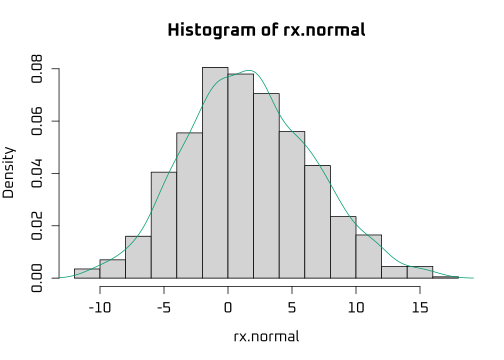
\includegraphics[width=\maxwidth]{figure/unnamed-chunk-13-1} 
\begin{kframe}\begin{alltt}
\hlkwd{hist}\hlstd{(r.alpha,} \hlkwc{breaks}\hlstd{=}\hlnum{20}\hlstd{)}
\end{alltt}
\end{kframe}
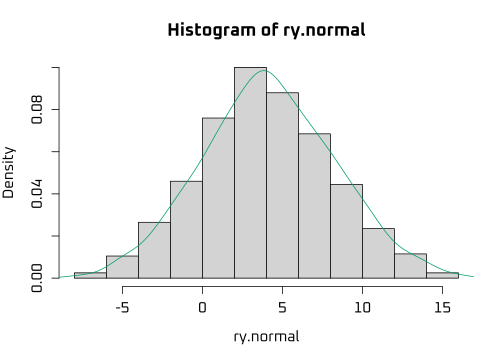
\includegraphics[width=\maxwidth]{figure/unnamed-chunk-13-2} 
\begin{kframe}\begin{alltt}
\hlkwd{ts.plot}\hlstd{(post.alpha)}
\end{alltt}
\end{kframe}
\includegraphics[width=\maxwidth]{figure/unnamed-chunk-13-3} 

\end{knitrout}
Ahora ilustramos el procedimiento de obtener la estimación de $\alpha$, $\beta$ y los $\theta_i$ usando suponiendo que se quiere estimar el número de accidentes de tránsito relacionados con motociclistas en las veinte localidades de la ciudad de Bogotá, suponga que en un mismo día determinado los números de estos accidentes son: $6, 5, 9, 2, 3, 0, 4, 1, 1, 2, 1, 6, 7, 2, 4, 3, 0, 4, 3, 2$.
\begin{knitrout}
\definecolor{shadecolor}{rgb}{0.933, 0.933, 0.933}\color{fgcolor}\begin{kframe}
\begin{alltt}
\hlstd{y} \hlkwb{<-} \hlkwd{c}\hlstd{(}\hlnum{6}\hlstd{,} \hlnum{5}\hlstd{,} \hlnum{9}\hlstd{,} \hlnum{2}\hlstd{,} \hlnum{3}\hlstd{,} \hlnum{0}\hlstd{,} \hlnum{4}\hlstd{,} \hlnum{1}\hlstd{,} \hlnum{1}\hlstd{,} \hlnum{2}\hlstd{,} \hlnum{1}\hlstd{,} \hlnum{6}\hlstd{,} \hlnum{7}\hlstd{,} \hlnum{2}\hlstd{,} \hlnum{4}\hlstd{,} \hlnum{3}\hlstd{,} \hlnum{0}\hlstd{,} \hlnum{4}\hlstd{,} \hlnum{3}\hlstd{,} \hlnum{2}\hlstd{)}
\hlstd{n} \hlkwb{<-} \hlkwd{length}\hlstd{(y)}
\hlstd{n.sim} \hlkwb{<-} \hlnum{1000}
\hlstd{res.theta} \hlkwb{<-} \hlkwd{matrix}\hlstd{(}\hlnum{NA}\hlstd{,n.sim,n); res.beta} \hlkwb{<-} \hlkwd{c}\hlstd{(); res.alpha} \hlkwb{<-} \hlkwd{c}\hlstd{()}
\hlcom{# Valor inicial para theta}
\hlstd{res.theta[}\hlnum{1}\hlstd{,]} \hlkwb{<-} \hlnum{20}
\hlcom{# Valor inicial para beta}
\hlstd{res.beta[}\hlnum{1}\hlstd{]} \hlkwb{<-} \hlnum{1}
\hlcom{# Simular un valor para alpha}
 \hlcom{# creación de la grilla para alpha}
 \hlstd{alpha.grid} \hlkwb{<-} \hlkwd{seq}\hlstd{(}\hlnum{0.05}\hlstd{,} \hlnum{20}\hlstd{,} \hlkwc{by}\hlstd{=}\hlnum{0.01}\hlstd{)}
 \hlstd{a} \hlkwb{<-} \hlstd{c} \hlkwb{<-} \hlnum{2}
 \hlstd{b} \hlkwb{<-} \hlstd{d} \hlkwb{<-} \hlnum{3}
 \hlcom{# probabilidad para cada valor en la grilla}
 \hlstd{post.alpha} \hlkwb{<-} \hlkwd{c}\hlstd{()}
 \hlkwa{for}\hlstd{(k} \hlkwa{in} \hlnum{1}\hlopt{:}\hlkwd{length}\hlstd{(alpha.grid))\{}
  \hlstd{post.alpha[k]} \hlkwb{<-} \hlkwd{post}\hlstd{(res.theta[}\hlnum{1}\hlstd{,], alpha.grid[k], res.beta[}\hlnum{1}\hlstd{],a,b)}
 \hlstd{\}}
 \hlstd{N.grid} \hlkwb{<-} \hlkwd{length}\hlstd{(post.alpha)}
 \hlstd{post.alpha} \hlkwb{<-} \hlstd{post.alpha}\hlopt{/}\hlkwd{sum}\hlstd{(post.alpha)}
 \hlstd{res.alpha[}\hlnum{1}\hlstd{]} \hlkwb{<-} \hlstd{alpha.grid[}\hlkwd{sample}\hlstd{(}\hlkwd{length}\hlstd{(alpha.grid),} \hlnum{1}\hlstd{,} \hlkwc{prob}\hlstd{=post.alpha,} \hlkwc{replace}\hlstd{=}\hlnum{TRUE}\hlstd{)]}
 \hlcom{# Aquí comienza a simular los valores de los parámetros}
 \hlkwa{for}\hlstd{(i} \hlkwa{in} \hlnum{2}\hlopt{:}\hlstd{n.sim)\{}
 \hlcom{# Simular un valor para theta}
   \hlkwa{for}\hlstd{(j} \hlkwa{in} \hlnum{1}\hlopt{:}\hlstd{n)\{}
     \hlstd{res.theta[i,j]} \hlkwb{<-} \hlkwd{rgamma}\hlstd{(}\hlnum{1}\hlstd{,} \hlkwc{shape}\hlstd{=y[j]}\hlopt{+}\hlstd{res.alpha[i}\hlopt{-}\hlnum{1}\hlstd{],} \hlkwc{rate}\hlstd{=res.beta[i}\hlopt{-}\hlnum{1}\hlstd{]}\hlopt{+}\hlnum{1}\hlstd{)}
   \hlstd{\}}
 \hlcom{# Simular un valor para beta}
   \hlstd{res.beta[i]} \hlkwb{<-} \hlkwd{rgamma}\hlstd{(}\hlnum{1}\hlstd{, n}\hlopt{*}\hlstd{(res.alpha[i}\hlopt{-}\hlnum{1}\hlstd{]}\hlopt{+}\hlstd{c}\hlopt{-}\hlnum{1}\hlstd{)}\hlopt{+}\hlnum{1}\hlstd{,} \hlkwc{rate}\hlstd{=n}\hlopt{*}\hlstd{d}\hlopt{+}\hlkwd{sum}\hlstd{(res.theta[i,]))}
 \hlcom{# Simular un valor para alpha}
 \hlstd{post.alpha} \hlkwb{<-} \hlkwd{c}\hlstd{()}
 \hlkwa{for}\hlstd{(k} \hlkwa{in} \hlnum{1}\hlopt{:}\hlkwd{length}\hlstd{(alpha.grid))\{}
  \hlstd{post.alpha[k]} \hlkwb{<-} \hlkwd{post}\hlstd{(res.theta[i,],alpha.grid[k],res.beta[i],a,b)}
 \hlstd{\}}
 \hlstd{post.alpha} \hlkwb{<-} \hlstd{post.alpha}\hlopt{/}\hlkwd{sum}\hlstd{(post.alpha)}

 \hlstd{res.alpha[i]} \hlkwb{<-} \hlstd{alpha.grid[}\hlkwd{sample}\hlstd{(}\hlkwd{length}\hlstd{(post.alpha),} \hlnum{1}\hlstd{,} \hlkwc{prob}\hlstd{=post.alpha,} \hlkwc{replace}\hlstd{=}\hlnum{TRUE}\hlstd{)]}
 \hlstd{\}}
 \hlcom{# Verificar la convergencia de algunos pará}
 \hlkwd{par}\hlstd{(}\hlkwc{mfrow}\hlstd{=}\hlkwd{c}\hlstd{(}\hlnum{2}\hlstd{,}\hlnum{2}\hlstd{))}
 \hlkwd{ts.plot}\hlstd{(res.theta[,}\hlnum{1}\hlstd{]);} \hlkwd{ts.plot}\hlstd{(res.theta[,}\hlnum{2}\hlstd{])}
 \hlkwd{ts.plot}\hlstd{(res.alpha);} \hlkwd{ts.plot}\hlstd{(res.beta)}
\end{alltt}
\end{kframe}
\includegraphics[width=\maxwidth]{figure/unnamed-chunk-14-1} 
\begin{kframe}\begin{alltt}
 \hlcom{# Calcular la estimación de los parámetros tomando la segunda mitad de los valores simulados}
 \hlkwd{colMeans}\hlstd{(res.theta[}\hlopt{-}\hlstd{(}\hlnum{1}\hlopt{:}\hlstd{(n.sim}\hlopt{/}\hlnum{2}\hlstd{)),])}
\end{alltt}
\begin{verbatim}
##  [1] 5.6 4.7 7.5 2.6 3.3 1.1 3.9 1.9 1.9 2.5 1.8 5.4 6.0 2.6 3.9 3.4 1.2
## [18] 3.8 3.2 2.6
\end{verbatim}
\begin{alltt}
 \hlkwd{mean}\hlstd{(res.alpha[}\hlopt{-}\hlstd{(}\hlnum{1}\hlopt{:}\hlstd{(n.sim}\hlopt{/}\hlnum{2}\hlstd{))])}
\end{alltt}
\begin{verbatim}
## [1] 1.7
\end{verbatim}
\begin{alltt}
 \hlkwd{mean}\hlstd{(res.beta[}\hlopt{-}\hlstd{(}\hlnum{1}\hlopt{:}\hlstd{(n.sim}\hlopt{/}\hlnum{2}\hlstd{))])}
\end{alltt}
\begin{verbatim}
## [1] 0.42
\end{verbatim}
\end{kframe}
\end{knitrout}

El anterior desarrollo teórico también se puede adaptar para el caso cuando se asume la misma media para todas las variables observadas, esto es, $Y_i\mid\theta$ para $i=1,\cdots,n$. En este caso, se tiene que 
\begin{equation*}
p(\theta,\alpha,\beta\mid\mathbf{Y})\propto e^{-(n+\beta)\theta}\theta^{\sum y_i+\alpha-1}\beta^{\alpha+c-1}e^{-\alpha b-\beta d}\alpha^{a-1}/\Gamma(\alpha)
\end{equation*}

de donde se puede concluir que 
\begin{align}
\theta\mid\alpha,\beta,\mathbf{Y}&\sim Gamma(\sum y_i+\alpha,n+\beta)\label{Poisson_Gamma1}\\
\alpha\mid\theta,\beta,\mathbf{Y}&\propto(\theta\beta)^\alpha e^{-\alpha b}\alpha^{a-1}/\Gamma(\alpha)\label{Poisson_Gamma2}\\
\beta\mid\theta,\alpha,\mathbf{Y}&\sim Gamma(\alpha+c,\theta+d)\label{Poisson_Gamma3}
\end{align}

\subsection{Modelo Normal}
Considere una variación de la estructura jerárquica de la sección \ref{Normal_Normal}, en donde las observaciones siguen el siguiente modelo de probabilidad
\begin{equation*}
Y_i \mid \theta_i \sim Normal(\theta_i,\sigma^2) \ \ \ \ \ \ \ i=1,\ldots,n
\end{equation*}

y el parámetro $\sigma^2$ se supone conocido. Sin embargo, la distribución previa para los parámetros de interés $\theta_i$ es
\begin{equation*}
\theta_i \mid \mu \sim Normal(\mu, \tau^2) \ \ \ \ \ \ \ i=1,\ldots,n
\end{equation*}
en donde los parámetros $\mu$ y $\tau^2$ son desconocidos. De esta forma, es necesario hallar una forma de estimar los valores de estos dos hiperparámetros, esto se puede llevar a cabo considerando diferente estructuras de dependencia entre $mu$ y $\tau^2$. 

\subsubsection{Hiperparámetros independientes}
En primer lugar, supongamos que los hiperparámetros son independientes en la distribución previa, es decir que su función de densidad conjunta se puede factorizar como el producto de las distribuciones marginales de cada uno de los hiperparámetros. Más aún, si se supone que las distribuciones previa marginales son no informativas y siguen una estructura probabilística uniforme, entonces se tiene que
\begin{equation*}
p(\mu,\tau^2)=p(\mu)p(\tau^2)\propto k
\end{equation*}

Con esta formulación se deduce que la distribución posterior conjunta condicional a una sola observación está dada por
\begin{align}
p(\theta_i,\mu,\tau^2 \mid Y_i) &\propto p(Y_i \mid \theta_i)p(\theta_i \mid \mu,\tau^2)p(\mu,\tau^2) \notag \\
&\propto p(Y_i \mid \theta_i)p(\theta_i \mid \mu,\tau^2) \notag \\
&\propto \exp\left\{\frac{1}{2\sigma^2}(y_i-\theta_i)^2\right\}
\frac{1}{\tau}\exp\left\{\frac{1}{2\tau^2}(\theta_i-\mu)^2\right\}
\end{align}

Y la distribución distribución posterior conjunta condicional a todas las observaciones y a todos los parámetros de interés es
\begin{align*}
p(\btheta,\mu,\tau^2 \mid \mathbf{Y})
&\propto p(\mathbf{Y} \mid \btheta)p(\btheta \mid \mu,\tau^2)  \\
&\propto \prod_{i=1}^n p(Y_i \mid \theta_i) \prod_{i=1}^n p(\theta_i \mid \mu,\tau^2)  \\
&\propto \exp\left\{\frac{1}{2\sigma^2}\sum_{i=1}^n(y_i-\theta_i)^2\right\}
\frac{1}{\tau^n}\exp\left\{\frac{1}{2\tau^2}\sum_{i=1}^n(\theta_i-\mu)^2\right\}
\end{align*}

Utilizaremos la técnica del condicionamiento para encontrar la distribución condicional del vector de parámetros de interés $\btheta$ y de los hiperparámetros. Por lo tanto se tiene que
\begin{align*}
p(\btheta \mid \mu,\tau^2,\mathbf{Y})
&\propto p(\btheta,\underbrace{\mu,\tau^2}_{fijos},\mathbf{Y})\\
p(\mu \mid \btheta,\tau^2,\mathbf{Y})
&\propto p(\mu,\underbrace{\btheta,\tau^2}_{fijos},\mathbf{Y}) \\
p(\tau^2 \mid \btheta,\mu,\mathbf{Y})
&\propto p(\mu,\underbrace{\btheta,\tau^2}_{fijos},\mathbf{Y})
\end{align*}

Con la anterior formulación se tiene la siguiente serie de resultados que dan cuenta de las distribuciones apropiadas para cada uno de los parámetros.

\begin{Res}
La distribución posterior del parámetro de interés $\theta_i$ es
\begin{equation*}
\theta_i\sim Normal(\mu_i,\tau_1^2)
\end{equation*}
en donde
\begin{equation*}
\mu_i=\frac{\frac{1}{\sigma^2}Y_i+\frac{1}{\tau^2}\mu}{\frac{1}{\sigma^2}+\frac{1}{\tau^2}}
\ \ \ \ \ \ \ \text{y} \ \ \ \ \ \ \
\tau_1^2=\left(\frac{1}{\sigma^2}+\frac{1}{\tau^2}\right)^{-1}
\end{equation*}
\end{Res}

\begin{proof}
Utilizando la técnica del condicionamiento posterior se tiene que
\begin{align*}
p(\theta_i \mid \mu,\tau^2,Y_i)
&\propto p(\theta_i,\underbrace{\mu,\tau^2}_{fijos},Y_i)\\
&\propto \exp\left\{-\frac{1}{2\sigma^2}(y_i-\theta_i)^2-\frac{1}{2\tau^2}(\theta_i-\mu)^2\right\}
\end{align*}
y utilizando el mismo razonamiento que en la demostración del Resultado 2.6.1 se encuentra una expresión idéntica a la función de distribución de una variable aleatoria con distribución $Normal(\mu_i,\tau_1^2)$.
\end{proof}

\begin{Res}
La distribución posterior del hiper-parámetro $\mu$ es
\begin{equation*}
\mu\sim Normal(\bar{\theta},\tau^2/n)
\end{equation*}
en donde $\bar{\theta}=\dfrac{1}{n}\sum_{i=1}^n\theta_i$.
\end{Res}

\begin{proof}
Utilizando la técnica del condicionamiento posterior y teniendo en cuenta que
\begin{equation*}
\sum_{i=1}^n(\theta_i-\mu)^2=\sum_{i=1}^n(\theta_i-\bar{\theta})^2+n(\mu-\bar{\theta})^2
\end{equation*}

entonces, se tiene que
\begin{align*}
p(\mu \mid \btheta,\tau^2,\mathbf{Y})
&\propto p(\mu,\underbrace{\btheta,\tau^2}_{fijos},\mathbf{Y})\\
&\propto \exp\left\{-\frac{1}{2\tau^2}\sum_{i=1}^n(\theta_i-\mu)^2\right\}
 \propto \exp\left\{-\frac{n}{2\tau^2}(\mu-\bar{\theta})^2\right\}
\end{align*}
Por lo tanto, factorizando convenientemente, se encuentra una expresión idéntica a la función de distribución de una variable aleatoria con distribución $Normal(\bar{\theta},\tau^2/n)$.
\end{proof}

\begin{Res}
La distribución posterior del hiper-parámetro $\tau^2$ es
\begin{equation*}
\tau^2 \sim Inversa-Gamma(n/2-1,nS^2_{\mu}/2)
\end{equation*}
en donde $nS^2_{\mu}=\sum_{i=1}^n(\theta_i-\mu)^2$.
\end{Res}

\begin{proof}
Utilizando la técnica del condicionamiento posterior se tiene que
\begin{align*}
p(\tau^2 \mid \btheta,\mu,\mathbf{Y})
&\propto p(\tau^2,\underbrace{\btheta,\mu}_{fijos},\mathbf{Y})\\
&\propto \frac{1}{\tau^n} \exp\left\{\frac{1}{2\tau^2}\sum_{i=1}^n(\theta_i-\mu)^2\right\}\\
&\propto \left(\tau^2\right)^{-n/2} \exp\left\{\frac{nS^2_{\mu}}{2\tau^2}\right\}
\end{align*}
Por lo tanto, factorizando convenientemente, se encuentra una expresión idéntica a la función de distribución de una variable aleatoria con distribución $Inversa-Gamma(n/2-1,nS^2_{\mu}/2)$.
\end{proof}

Utilizando un algoritmo que genere una cadena de Markov, y utilizando los anteriores resultados se realiza un análisis bayesiano propiamente dicho.

Ilustramos la implementación en \verb'R' a continuación para datos de $y$ de 5.8, 4.7, 7.0, 8.3, 3.7, 3.7, 5.5, 7.7, 6.7 y 6.7.
\begin{knitrout}
\definecolor{shadecolor}{rgb}{0.933, 0.933, 0.933}\color{fgcolor}\begin{kframe}
\begin{alltt}
\hlkwd{library}\hlstd{(pscl)}
\hlstd{y} \hlkwb{<-} \hlkwd{c}\hlstd{(}\hlnum{5.8}\hlstd{,} \hlnum{4.7}\hlstd{,} \hlnum{7.0}\hlstd{,} \hlnum{8.3}\hlstd{,} \hlnum{3.7}\hlstd{,} \hlnum{3.7}\hlstd{,} \hlnum{5.5}\hlstd{,} \hlnum{7.7}\hlstd{,} \hlnum{6.7}\hlstd{,} \hlnum{6.7}\hlstd{)}
\hlstd{n} \hlkwb{<-} \hlkwd{length}\hlstd{(y); sigma2} \hlkwb{<-} \hlnum{1}
\hlstd{n.sim} \hlkwb{<-} \hlnum{1000}
\hlstd{res.mu} \hlkwb{<-} \hlkwd{rep}\hlstd{(}\hlnum{0}\hlstd{, n.sim); res.tau2} \hlkwb{<-} \hlkwd{rep}\hlstd{(}\hlnum{1}\hlstd{, n.sim); res.theta}\hlkwb{<-} \hlkwd{matrix}\hlstd{(}\hlnum{NA}\hlstd{, n.sim, n)}
\hlcom{# Simular el primer valor para theta}
\hlstd{tau2_1} \hlkwb{<-} \hlstd{(sigma2}\hlopt{^-}\hlnum{1} \hlopt{+} \hlstd{res.tau2[}\hlnum{1}\hlstd{]}\hlopt{^-}\hlnum{1}\hlstd{)}\hlopt{^-}\hlnum{1}
\hlstd{mu_i} \hlkwb{<-} \hlstd{(y}\hlopt{/}\hlstd{sigma2} \hlopt{+} \hlstd{res.mu[}\hlnum{1}\hlstd{]}\hlopt{/}\hlstd{res.tau2[}\hlnum{1}\hlstd{])}\hlopt{*}\hlstd{tau2_1}
\hlstd{res.theta[}\hlnum{1}\hlstd{,]} \hlkwb{<-} \hlkwd{rnorm}\hlstd{(}\hlnum{1}\hlstd{, mu_i,} \hlkwd{sqrt}\hlstd{(tau2_1))}
\hlcom{# Aquí comienza a simular valores para todos los parámetros}
\hlkwa{for}\hlstd{(i} \hlkwa{in} \hlnum{2}\hlopt{:}\hlstd{n.sim)\{}
  \hlstd{res.mu[i]} \hlkwb{<-} \hlkwd{rnorm}\hlstd{(}\hlnum{1}\hlstd{,} \hlkwd{mean}\hlstd{(res.theta[i}\hlopt{-}\hlnum{1}\hlstd{,]),} \hlkwd{sqrt}\hlstd{(res.tau2[i}\hlopt{-}\hlnum{1}\hlstd{]}\hlopt{/}\hlstd{n))}
  \hlstd{res.tau2[i]} \hlkwb{<-} \hlkwd{rigamma}\hlstd{(}\hlnum{1}\hlstd{,} \hlkwc{alpha}\hlstd{=n}\hlopt{/}\hlnum{2}\hlopt{-}\hlnum{1}\hlstd{,} \hlkwc{beta}\hlstd{=}\hlkwd{sum}\hlstd{((res.theta[i}\hlopt{-}\hlnum{1}\hlstd{,]}\hlopt{-}\hlstd{res.mu[i])}\hlopt{^}\hlnum{2}\hlstd{)}\hlopt{/}\hlnum{2}\hlstd{)}
  \hlstd{tau2_1} \hlkwb{<-} \hlstd{(sigma2}\hlopt{^-}\hlnum{1} \hlopt{+} \hlstd{res.tau2[i]}\hlopt{^-}\hlnum{1}\hlstd{)}\hlopt{^-}\hlnum{1}
  \hlstd{mu_i} \hlkwb{<-} \hlstd{(y}\hlopt{/}\hlstd{sigma2} \hlopt{+} \hlstd{res.mu[i]}\hlopt{/}\hlstd{res.tau2[i])}\hlopt{*}\hlstd{tau2_1}
  \hlkwa{for}\hlstd{(j} \hlkwa{in} \hlnum{1}\hlopt{:}\hlstd{n)\{}
    \hlstd{res.theta[i,j]} \hlkwb{<-} \hlkwd{rnorm}\hlstd{(}\hlnum{1}\hlstd{, mu_i[j],} \hlkwd{sqrt}\hlstd{(tau2_1))}
  \hlstd{\}}
\hlstd{\}}
 \hlcom{# Verificar la convergencia de algunos pará}
 \hlkwd{par}\hlstd{(}\hlkwc{mfrow}\hlstd{=}\hlkwd{c}\hlstd{(}\hlnum{2}\hlstd{,}\hlnum{2}\hlstd{))}
 \hlkwd{ts.plot}\hlstd{(res.theta[,}\hlnum{1}\hlstd{]);} \hlkwd{ts.plot}\hlstd{(res.theta[,}\hlnum{2}\hlstd{])}
 \hlkwd{ts.plot}\hlstd{(res.mu);} \hlkwd{ts.plot}\hlstd{(res.tau2)}
\end{alltt}
\end{kframe}
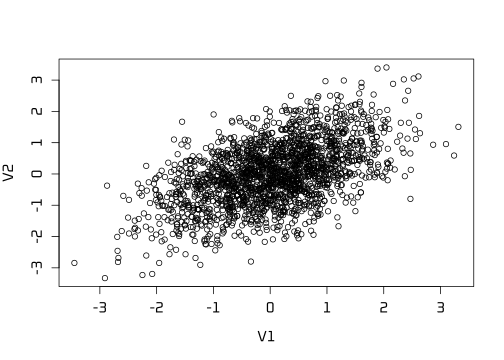
\includegraphics[width=\maxwidth]{figure/unnamed-chunk-15-1} 
\begin{kframe}\begin{alltt}
 \hlcom{# Calcular la estimación de los parámetros tomando la segunda mitad de los valores simulados}
 \hlkwd{colMeans}\hlstd{(res.theta[}\hlopt{-}\hlstd{(}\hlnum{1}\hlopt{:}\hlstd{(n.sim}\hlopt{/}\hlnum{2}\hlstd{)),])}
\end{alltt}
\begin{verbatim}
##  [1] 6.0 5.1 6.6 7.5 4.4 4.5 5.7 7.1 6.5 6.5
\end{verbatim}
\begin{alltt}
 \hlkwd{mean}\hlstd{(res.mu[}\hlopt{-}\hlstd{(}\hlnum{1}\hlopt{:}\hlstd{(n.sim}\hlopt{/}\hlnum{2}\hlstd{))])}
\end{alltt}
\begin{verbatim}
## [1] 6
\end{verbatim}
\begin{alltt}
 \hlkwd{mean}\hlstd{(res.tau2[}\hlopt{-}\hlstd{(}\hlnum{1}\hlopt{:}\hlstd{(n.sim}\hlopt{/}\hlnum{2}\hlstd{))])}
\end{alltt}
\begin{verbatim}
## [1] 3.1
\end{verbatim}
\end{kframe}
\end{knitrout}


\subsubsection{Hiperparámetros dependientes}

Siguiendo el algoritmo dado al comienzo de esta sección, en dónde se dan los lineamentos generales para realizar un análisis jerárquico. En primer lugar se debe considerar la distribución posterior de los parámetros, que en este caso depende de la distribución previa de los hiperparámetros.

Suponga entonces, al igual que en capítulos anteriores, que los hiperparámetros son dependientes a una vía. Es decir, que $\mu$ depende de $\tau^2$ pero que $\tau^2$ no depende de $\mu$. En estos términos, la distribución previa de los hiperparámetros está dada por
\begin{equation*}
p(\mu,\tau^2)=p(\mu \mid \tau^2)p(\tau^2)
\end{equation*}

Luego, siguiendo la regla de bayes y suponiendo que los hiperparámetros son condicionalmente independientes de las observaciones dado el vector de parámetros de interés, la distribución posterior del vector de parámetros de interés $\btheta=(\theta_1,\ldots,\theta_n)'$ y de los hiperparámetros $\mu, \tau^2$ es
\begin{align*}
p(\btheta,\mu,\tau^2 \mid \mathbf{Y})
&\propto p(\mathbf{Y} \mid \btheta)p(\btheta \mid \mu,\tau^2)p(\mu,\tau^2)  \\
&\propto p(\mu,\tau^2) \prod_{i=1}^n p(Y_i \mid \theta_i) \prod_{i=1}^n p(\theta_i \mid \mu,\tau^2)  \\
&\propto p(\mu,\tau^2) \exp\left\{\frac{-1}{2\sigma^2}\sum_{i=1}^n(y_i-\theta_i)^2\right\}
\frac{1}{\tau^n}\exp\left\{\frac{-1}{2\tau^2}\sum_{i=1}^n(\theta_i-\mu)^2\right\}
\end{align*}

Con base en lo anterior, se tienen el siguiente resultado para el análisis bayesiano jerárquico de un sólo componente $\theta_i$ de $\btheta$.

\begin{Res}
La distribución posterior del componente $\theta_i$ perteneciente al vector de parámetros de interés $\btheta$ es
\begin{equation*}
\theta_i\sim Normal(\mu_i,\tau_1^2)
\end{equation*}
en donde
\begin{equation*}
\mu_i=\frac{\frac{1}{\sigma^2}Y_i+\frac{1}{\tau^2}\mu}{\frac{1}{\sigma^2}+\frac{1}{\tau^2}}
\ \ \ \ \ \ \ \text{y} \ \ \ \ \ \ \
\tau_1^2=\left(\frac{1}{\sigma^2}+\frac{1}{\tau^2}\right)^{-1}
\end{equation*}
\end{Res}

\begin{proof}
La prueba del resultado es inmediata al considerar la técnica del condicionamiento posterior como en la demostración del Resultado 4.2.1. puesto que
\begin{align*}
p(\theta_i \mid \mu,\tau^2,Y_i)&\propto
p(\theta_i,\underbrace{\mu,\tau^2}_{fijos} \mid Y_i)\\
&\propto
p(Y_i \mid \theta_i)p(\theta_i \mid \mu,\tau^2)p(\mu,\tau^2)\\
&\propto
(Y_i \mid \theta_i)p(\theta_i \mid \mu,\tau^2)
\end{align*}
\end{proof}

siguiendo con el algoritmo del análisis jerárquico, el siguiente paso corresponde a la determinación de la distribución posterior de los hiperparámetros $\mu, \tau^2$ la cual, suponiendo que la distribución previa conjunta para ambos hiperparámetros es uniforme y no informativa, está dada por el Resultado 4.1.1.
\begin{align*}
p(\mu, \tau^2 \mid \mathbf{Y})&\propto p(\mu,\tau^2)p(\mathbf{Y} \mid \mu,\tau^2)\\
&\propto \prod_{i=1}^n p(Y_i \mid \mu,\tau^2))\\
&\propto \prod_{i=1}^n Normal(\mu,\tau^2+\sigma^2)
\end{align*}

Ahora, por otro lado, el análisis individual de los hiperparámetros está regido por la siguiente expresión
\begin{align*}
p(\mu, \tau^2 \mid \mathbf{Y})=p(\mu \mid  \tau^2,\mathbf{Y})p(\tau^2 \mid \mathbf{Y})
\end{align*}

En este orden de ideas, se tienen los siguientes resultados acerca de la distribución posterior para $\mu$ dada por $p(\mu \mid  \tau^2,\mathbf{Y})$ y para $\tau^2$ dada por $p(\tau^2 \mid \mathbf{Y})$

\begin{Res}
La distribución posterior del hiperparámetro $mu$ condicionada a $\tau^2,\mathbf{Y}$ es
\begin{equation*}
\mu \mid \tau^2,\mathbf{Y} \sim Normal \left(\hat{\mu},\hat{\tau}^2\right)
\end{equation*}
donde $\hat{\mu}=\bar{Y}$ y $n\hat{\tau}^2=\sigma^2+\tau^2$.
\end{Res}

\begin{proof}
Utilizando la técnica del condicionamiento posterior, nótese que la distribución posterior de $mu$ toma la siguiente forma

\begin{align*}
p(\mu \mid \tau^2,\mathbf{Y})&\propto p(\mu,\underbrace{\tau^2}_{fijo} \mid \mathbf{Y}) \\
&\propto \prod_{i=1}^n Normal(\mu,\tau^2+\sigma^2)
\end{align*}

Partiendo de este hecho, es fácil confirmar que

\begin{align*}
p(\mu \mid \tau^2,\mathbf{Y})&\propto
&\propto \exp\left\{\frac{1}{2(\sigma^2+\tau^2)}\sum_{i=1}^n(y_i-\mu)^2\right\}\\
&= \exp\left\{\frac{1}{2(\sigma^2+\tau^2)}\sum_{i=1}^n(y_i^2-2\mu Y_i+\mu^2)\right\}\\
&\propto \exp\left\{\frac{n}{2(\sigma^2+\tau^2)}(\mu^2-2\mu\bar{Y})\right\}\\
&\propto \exp\left\{\frac{n}{2(\sigma^2+\tau^2)}(\mu-\bar{Y})^2\right\}
\end{align*}
Por lo tanto, factorizando convenientemente, se encuentra una expresión idéntica a la
función de distribución de una variable aleatoria con distribución $Normal(\hat{\mu},\hat{\tau}^2)$.
\end{proof}

\begin{Res}
La distribución posterior del hiperparámetro $\tau$ es
\begin{equation*}
p(\tau^2 \mid \mathbf{Y})
\propto \sqrt{\hat{\tau}} \prod_{i=1}^n (\sigma^2+\tau^2)^{-1/2}\exp\left\{-\frac{1}{2(\sigma^2+\tau^2)}(y_i-\hat{\mu})^2\right\}
\end{equation*}
\end{Res}

\begin{proof}
En primer lugar, nótese que
\begin{align*}
p(\tau \mid \mathbf{Y})&= \frac{p(\mu,\tau^2 \mid \mathbf{Y})}{p(\mu \mid \tau^2,\mathbf{Y})}
\ \ \ \ \ \ \ \ \ \ \ \ \ \ \ \forall \mu \\
&\propto \frac{\prod_{i=1}^n Normal(\mu,\sigma^2+\tau^2)}{Normal(\hat{\mu},\hat{\tau}^2)}
\ \ \ \ \ \ \ \ \ \ \ \ \ \ \ \forall \mu
\end{align*}

La anterior igualdad debe mantenerse para cualquier valor de $\mu$; en particular se debe mantener para $\mu=\hat{\mu}$ \cite{Gelman03}. Por tanto,
\begin{align*}
p(\tau \mid \mathbf{Y}) &\propto \frac{Normal(\hat{\mu},\sigma^2+\tau^2)}{Normal(\hat{\mu},\hat{\tau}^2)}\\
&\propto \frac{\prod_{i=1}^n Normal(\hat{\mu},\sigma^2+\tau^2)}{Normal(\hat{\mu},\hat{\tau}^2)}\\
&\propto \sqrt{\hat{\tau}}\prod_{i=1}^n (\sigma^2+\tau^2)^{-1/2}\exp\left\{-\frac{1}{2(\sigma^2+\tau^2)}(y_i-\hat{\mu})^2\right\} \exp\left\{\frac{1}{2\hat{\tau}^2}(\hat{\mu}-\hat{\mu})^2\right\}\\
&\propto \sqrt{\hat{\tau}}\prod_{i=1}^n (\sigma^2+\tau^2)^{-1/2}\exp\left\{-\frac{1}{2(\sigma^2+\tau^2)}(y_i-\hat{\mu})^2\right\}
\end{align*}
\end{proof}

En términos de simulación, los anteriores resultados garantizan una estructura formal que permita simular la distribución posterior del hiperparámetro $\tau^2$, y mediante esta encontrar una estimación para reemplazarla en la distribución posterior del hiperparámetro $\mu$ y repetir el proceso anterior. Con estos valores bien definidos, entonces utilizar el Resultado 4.2.4 para proseguir con el análisis bayesiano clásico. 

\section{Ejercicios}
\begin{enumerate}
\item Para el modelo $Y_i\sim\theta_i Normal(\theta_i,\sigma^2)$ para $i=1,\cdots,n$ del modelo Normal-Normal, desarrollando $E(Y_i)$, encuentra que $\mu$ se peude calcular como $\bar{y}$.
\item Demustre las ecuaciones \ref{Poisson_Gamma1}, \ref{Poisson_Gamma2} y \ref{Poisson_Gamma3}. Modifique los códigos del caso $Y_i\mid\theta_i\sim Poisson(\theta_i)$ para estimar $\alpha$, $\beta$ y $\theta$, y aplíquelos a los datos del ejemplo \ref{Datos_Poisson} asumiendo (i) $\alpha=\beta=0.1$ y (ii) $\alpha=\beta=10$. Cómo afectan los valores de $\alpha$ y $\beta$ sobre la estimación final de $\theta$?
\end{enumerate}
